\documentclass[review,nonacm,screen,acmsmall,anonymous=true]{acmart}
\settopmatter{printfolios=true,printccs=true,printacmref=true}

\bibliographystyle{ACM-Reference-Format}
\citestyle{acmauthoryear}   %% For author/year citations
\usepackage{listings,multirow,wrapfig,xspace}
\usepackage{xcolor,tikz,graphicx, pifont}
%\usetikzlibrary{positioning}

\newcommand{\authorcomment}[3]{\xspace\textcolor{#1}{{\bf #2} #3}\xspace}
% For author notes:
\newcommand{\AG}[1]{\authorcomment{orange}{AG}{#1}}
\newcommand{\JV}[1]{\authorcomment{red}{JV}{#1}}
\newcommand{\JJ}[1]{\authorcomment{green}{JJ}{#1}}
\newcommand{\SK}[1]{\authorcomment{yellow}{SK}{#1}}
\newcommand{\OF}[1]{\authorcomment{magenta}{OF}{#1}}

% For meta comments:
\newcommand{\isit}[1]{\authorcomment{cyan}{Check}{#1}}
\newcommand{\todo}[1]{\authorcomment{red}{TODO}{#1}}
\newcommand{\xmark}{\textcolor{red}{\ding{55}}}
\newcommand{\cmark}{\textcolor{green}{\ding{51}}}

\newcommand{\always}{\emph{Always}\xspace}
\newcommand{\sometimes}{\emph{Sometimes}\xspace}
\newcommand{\sometimesStar}{\emph{Sometimes*}\xspace}
\newcommand{\never}{\emph{Never}\xspace}
\newcommand{\neverStar}{\emph{Never*}\xspace}
\newcommand{\rdyn}{{\sf R-dyntrace}\xspace}
\newcommand{\instr}{{\sf InstrumentR}\xspace}

\lstset{language=R}

\definecolor{LightGray}{RGB}{247, 247, 247}
\definecolor{Gray}{rgb}{.3,.3,.3}
\definecolor{DarkGray}{rgb}{.5,.5,.5}

\lstset{ %
  columns=flexible,
  captionpos=b,
  frame=single,
  framerule=0pt,
  framexleftmargin=1mm,
  framexrightmargin=1mm,
  tabsize=2,
  belowskip=0pt,
  basicstyle=\small\ttfamily,
  backgroundcolor=\color{LightGray},
  emphstyle=\sffamily,
  keywordstyle=\bfseries,
  commentstyle=\color{Gray}\em,
  stringstyle=\color{Gray}
}
\lstdefinestyle{R}{ %
  language=R,
  deletekeywords={new, env, equal, c, runif, trace, args, exp, t, all, get,body,
    names, is, environment, class, substitute, expression, list, null, Internal,
    sample, diag, length, rep, nrow, stop, offset, pmax, Machine,check,names,merge,all,
    double, parent, frame, par, methods, end, dir, apply, deparse, missing,any,
    plot, as, integer, character, inherits, numeric, paste, eval, quote, call,
    formula, df, log, sum, c, local, legend, file, scale, round, title, order,
    drop, which, grid, print, ncol, dim, max, format, sort, rug, matrix, start,
    unique, mean, df, attr, do, power},
  otherkeywords={},
  breaklines=true
}

\newcommand{\code}[1]{\lstinline[style=R]|#1|\xspace}
\renewcommand{\c}[1]{\lstinline[style=R]|#1|\xspace}
\newcommand{\strictr}{{\sf StrictR}\xspace}
\newcommand{\lazr}{{\sf LazR}\xspace}
\renewcommand{\Rsh}{{\sf\u R}\xspace}
\newcommand{\Rshstrict}{{\sf\u R-strict}\xspace}

\newcommand{\eg}{\emph{e.g.},\xspace}
\newcommand{\ie}{\emph{i.e.},\xspace}

%% Performance evaluation results:

\newcommand{\benchmarkSuiteSize}{14\xspace}

%% Baseline perf  Gnur - Rsh (1x15)  
%% https://rir-benchmarks.prl.fit.cvut.cz/diff?warmup=5&kind=diff&job_ids%5B%5D=1169772175&job_ids%5B%5D=1169772178&selection=promisebreaker
\newcommand{\speedupRsh}{$1.89\times$\xspace}
\newcommand{\speedupRshMax}{$56\times$\xspace}
\newcommand{\speedupRshMin}{$0.64\times$\xspace}

%%  Speedup  Rsh - Rsh strict (4x25)  
%% https://rir-benchmarks.prl.fit.cvut.cz/diff?warmup=5&kind=diff&job_ids%5B%5D=1174881563&job_ids%5B%5D=1174869738&execution=all&selection=promisebreaker
\newcommand{\speedupRshStrict}{$1.17\times$\xspace}
\newcommand{\speedupRshStrictMax}{$1.95\times$\xspace}
\newcommand{\speedupRshStrictMin}{$0.92\times$\xspace}
\newcommand{\speedupRshStrictSignificant}{9\xspace}  %% *** TODO: WHAT DOES SIGNIFICANT MEAN? **

%%  Speedup BC  (1x15) 
%% https://rir-benchmarks.prl.fit.cvut.cz/diff?warmup=5&kind=diff&job_ids%5B%5D=1172677834&job_ids%5B%5D=1172663147&selection=promisebreaker
\newcommand{\speedupBCRshStrict}{$1.16\times$\xspace}
\newcommand{\speedupBCRshStrictMax}{$1.48\times$\xspace}
\newcommand{\speedupBCRshStrictMin}{$1.00\times$\xspace}

%%  How much is BC slower?
%% https://rir-benchmarks.prl.fit.cvut.cz/diff?warmup=5&kind=diff&job_ids%5B%5D=1174869738&job_ids%5B%5D=1172663147&execution=all&selection=promisebreaker
\newcommand{\rshBCSlowdown}{$0.38\times$\xspace}

%% Reduction in promise allocation:
%% promise numbers using 1x15 iterations
\newcommand{\promiseAlocationReductionGnurRsh}{$91\%$\xspace}  %% 91.3 
\newcommand{\promiseAlocationReductionRshStrict}{$96\%$\xspace}  %%   95.6  OK (excluding fastaredux and fannkuchredux)
\newcommand{\promiseAlocationReductionGnurRshStrict}{$99\%$\xspace}   %%  99.33  (excluding fastaredux and fannkuchredux) 
\newcommand{\promiseAlocationReductionRshStrictToZero}{$2$\xspace}  %% OK (fastaredux and fannkuchredux drop to 0)
\newcommand{\promiseAlocationReductionGnurRshStrictMin}{$9.5\%$\xspace}  %% OK

%% time in GC in  Ř-strict / time in GC in Ř
\newcommand{\speedupGCRshStrictMax}{$190\%$\xspace}
\newcommand{\speedupGCRshStrictMin}{$50\%$\xspace}

%% How much is due to reduced allocation
%% https://rir-benchmarks.prl.fit.cvut.cz/diff?warmup=5&kind=diff&job_ids%5B%5D=1183876408&job_ids%5B%5D=1172677834&job_ids%5B%5D=1172663147&selection=promisebreaker
\newcommand{\speedupBCRshStrictAlloc}{$1.1\times$\xspace}
\newcommand{\speedupDueToReducedGC}{$38\%$\xspace}


\newcommand{\robustnesResult}{$0.56\%$\xspace}


%%% \setcopyright{rightsretained}
%%% \acmPrice{}
%%% \acmDOI{10.1145/3360579}
%%% \acmYear{2019}
%%% \copyrightyear{2019}
%%% \acmJournal{PACMPL}
%%% \acmVolume{3}
%%% \acmNumber{OOPSLA}
%%% \acmArticle{153}
%%% \acmMonth{10}
\begin{document}
\title{Promises Are Made To Be Broken}
\subtitle{Migrating the R ecosystem to strict evaluation semantics}

\author{Aviral Goel}\affiliation{\institution{Northeastern University}\country{USA}}
\author{Jan Ječmen}\affiliation{\institution{Czech Technical University}\country{Czechia}}
\author{Sebastián Krynski}\affiliation{\institution{Czech Technical University}\country{Czechia}}
\author{Olivier Flückiger}\affiliation{\institution{Northeastern University}\country{USA}}
\author{Jan Vitek}\affiliation{\institution{Czech Technical University and Northeastern University}\country{USA}}
\authorsaddresses{}
\renewcommand{\shortauthors}{Goel, Vitek}

\begin{abstract}
  Function calls in the R language do not evaluate their arguments; these are
  passed as suspended computations to the callee which evaluates them only if
  they are needed. After 25 years of experience with the language, there are
  very few cases where programmers leverage delayed evaluation intentionally.
  Yet, being lazy comes at a price in performance and complexity. This paper
  explores how one could evolve the semantics of the language towards strictness
  by default and laziness on demand. To provide a migration path, it is
  necessary to change the semantics of the language implementations and provide
  tooling for developers to migrate the libraries and user code in a way that
  does not introduce errors. This paper reports on a dynamic analysis that
  infers strictness signatures for functions and capture both intentional and
  accidental laziness. To assess the robustness of the inferred signatures, we
  implemented a source-to-source refactoring that forces the evaluation of
  arguments that have been annotated as strict. Finally, we report on the
  performance benefits of migration by extending a just-in-time compiler with
  support for strictness annotations.
\end{abstract}

\begin{CCSXML}
<ccs2012>
<concept>
<concept_id>10002944.10011123.10010912</concept_id>
<concept_desc>General and reference~Empirical studies</concept_desc>
<concept_significance>500</concept_significance>
</concept>
<concept>
<concept_id>10011007.10011006.10011008</concept_id>
<concept_desc>Software and its engineering~General programming languages</concept_desc>
<concept_significance>500</concept_significance>
</concept>
<concept>
<concept_id>10011007.10011006.10011050.10010517</concept_id>
<concept_desc>Software and its engineering~Scripting languages</concept_desc>
<concept_significance>500</concept_significance>
</concept>
<concept>
<concept_id>10011007.10011006.10011039.10011311</concept_id>
<concept_desc>Software and its engineering~Semantics</concept_desc>
<concept_significance>300</concept_significance>
</concept>
</ccs2012>
\end{CCSXML}

\ccsdesc[500]{General and reference~Empirical studies}
\ccsdesc[500]{Software and its engineering~General programming languages}
\ccsdesc[500]{Software and its engineering~Scripting languages}
\ccsdesc[300]{Software and its engineering~Semantics}

\keywords{R language, delayed or lazy evaluation}

\maketitle
\section{Introduction}

The R programming language is widely used in data science. Unbeknownst to many
of its end-users, function calls have a lazy semantics: arguments are suspended
computations which are evaluated if and when they are needed. \citet{oopsla19b}
provided a thorough observational study of a corpus consisting of 16,707
packages written in R. For the most part, the corpus appears to have been
written without reliance on laziness with the exception of code that leverages
it for meta-programming. This paper argues that laziness should be the exception
in R. We propose to make it a \emph{eager by default, lazy on demand} language
by introducing strictness annotations. The question we wish to answer is whether
it is possible to switch the semantics of a language without causing undue
breakage in the legacy code that is in daily use. This concern is relevant
because, even if programmers don't avail themselves of laziness, it is
conceivable that their code accidentally depends on it. A change in the order of
evaluation of arguments may introduce errors if that code was performing side
effects.

\paragraph{The case for strictness.} Laziness is error-prone, inconsistent
and costly! The combination of delayed evaluation and side-effects in a language
without type annotations is an invitation to subtle programming errors. If a
function has multiple evaluation orders and is called with effectful arguments,
their effects will be observed to happen in various orders. Functional languages
prevent ordering issues by reflecting effects in the type system. R cannot do
this as it is dynamically typed. Instead, libraries routinely add code at the
boundaries of their interface to force a single evaluation order. The design and
use of laziness is inconsistent because there are multiple points where
evaluation is arbitrarily forced. These include right-hand side of assignments
and function returns, neither of which is required in a lazy language.
Furthermore, to support object-oriented programming, R allows both single- and
multiple-dispatch; in order to perform dispatch, arguments must be evaluated
eagerly. Last, there are costs to lazy evaluation. Each argument must be boxed
in a data structure that holds a reference to the expression to evaluate, its
environment and the result of evaluation. Allocating and deallocating these data
structures put pressure on the memory manager. Delayed evaluation further
complicates the work of compilers for the language by hindering optimizations
and increasing the number of indirect calls.

\paragraph{The case for laziness.} The success of a programming language
often comes down to the strength of its ecosystem. With tens of millions of
lines of contributed library code, any change to the core semantics of the
language risks changing the behavior of some library functions. Preserving the
status quo is a pragmatic choice to protect the investment in legacy code bases.
There is also a genuine need for lazy evaluation, it is the building block of
the meta-programming facilities of the language. Unevaluated arguments can be
coerced back to their source code, that code can be modified, and evaluated in
an environment of the programmer's choice. Meta-programming is used to extend
the language and to create embedded domain specific languages. While it is
possible to imagine using macros instead, the number of libraries that use
meta-programming is sufficiently large that it would be non-trivial to refactor
them.

\paragraph{A pragmatic path forward.} How can an entire ecosystem migrate to
a new semantics? A viable migration path should follow the following four
tenets: ({\bf T1}) source code changes to legacy code should be kept to a
minimum; ({\bf T2}) the migration should either be (semi-)automated, and require
limit involvement of legacy developers; ({\bf T3}) the migration should have
measurable benefits; and ({\bf T4}) the migration should be testable with
discrepancies easily attributed to a specific change.
%
%
We propose a migration path that will lead to a mostly strict ecosystem based on
an augmented semantics for R, an performant implementation of that semantics in
the \Rsh compiler, and \lazr a tool for inferring strictness signatures.
Specifically, we propose an approach that follows the above guidelines.
\begin{itemize}
\item[{\bf T1:}] The extensions to the semantics are designed to be
  non-invasive, in our first iteration, only file that have functions requiring
  some of their arguments to be lazy need annotations, and these annotations can
  be added out of line in separate signature files. As the annotation are on
  functions, the need for those will be mostly focused at library interfaces.
  End-user code can remain unchanged. We claim that the behavior most R users
  expect from their code closely aligns to a strict semantics. This change will
  thus not affect their experience.
\item[{\bf T2:}] A tool can leverage the structure of the R ecosystem to infer
  annotations for legacy library code. R packages are hosted in a curated
  repository called CRAN, that repository enforce format and checks on the code
  stored in it. In particular every program has runnable use-cases and tests.
  The can use those to infer signatures for all packages. The inferred signature
  must be validated by a developer (or they can also be deployed and refined
  iteratively).
\item[{\bf T3:}] To evaluate the performance and memory benefits of decreasing
  the laziness of R programs, the an optimizing compiler can be extended to
  support strictness signatures. This will lead to code that performs fewer
  allocations, thus needs less frequent garbage collection passes, and can
  optimize evaluation of arguments by inlining it at the call site.
\item[{\bf T4:}] To test the robustness of inferred signatures to different
  calling contexts, each package can be tested by running the transitive closure
  of its clients and their tests. Programs that crash or departed from their
  expected behavior indicate erroneous strictness annotations.
\end{itemize}

Our long term aim is to propose such a migration path to the R community. In
this paper we propose to evaluate the proposed migration path. We make
the following contributions:

\begin{itemize}
\item We propose \strictr, a non-invasive extension of the R language, where
  optional signature files specify, for individual functions, which of their
  arguments are strict. The proposal is integrated in the R environment and
  compatible with the package loading model. In GNUR, the reference
  implementation of the language, the new semantics is implemented by
  source-to-source rewriting of functions as they created in the interpreter.
\item We implement \lazr, an infrastructure for large-scale inference of
  strictness signatures for legacy libraries. We evaluate \lazr on packages
  hosted in the CRAN repository. For each package \lazr extracts all executable
  code from vignettes, examples and tests, and infers signatures for all
  functions defined by the package. The process is shown to scale to the 500
  most widely used packages in the R ecosystem.
\item We conducted an experiment using the \Rsh optimizing just-in-time compiler
  to evaluate the benefits of unboxing and inlining
  delayed evaluation on a benchmark suite of small computational tasks. We show
  a median \speedupRshStrict speed up on those benchmarks.
\item We evaluate the robustness of the inferred signatures by testing them with
  2,000 packages that are transitive clients of the packages for which
  signatures were inferred. We report 0.3\% error rate, \emph{i.e.}~signatures
  that cause executions to diverge from the reference semantics.
\end{itemize}

Our conclusions are that a semi-automated migration is viable; for community
review we intend to reduce the error rate by folding all clients of packages
together to infer combined signatures.

\paragraph{Availability} Our work is in open source, all experiments are
repeatable and will be submitted for artifact evaluation.

\section{Background}

This section sets the stage by introducing related work and giving a brief
overview of R.

\subsection{Related Work}

There are three clusters of related results: research on adding and removing
laziness in functional languages, research on the R language, and approaches to
language migration.

\paragraph{Call by need}  Functional languages with
a call by need evaluation strategy must contend with memory pressure and
associated performance issues due to allocation of substantial numbers of thunks
(suspended computations)~\cite{transformopt,stricteffective,opteval}. While most
Haskell programs benefit from the strictness analysis pass performed by the
compiler. Due to its conservative nature, this pass misses some opportunities
for optimizations. To recover performance programmers can manually insert
strictness annotations to control evaluation but identifying where to put them
can be challenging. \citet{autobahn} proposed, Autobahn, a tool that
automatically infers strictness annotations using a genetic algorithm. The
approach relies on a dynamic analysis, as it does not approximate and cannot
guarantee termination on all inputs. As the annotations are based on a
heuristic, developers must manually validate their soundness. The authors report
an average 8.5\% speedup (with a maximum speed up of 89\%). \citet{lazyprof}
solve the complementary problem of suggesting laziness annotations for
call-by-value $\lambda$ calculus using a dynamic analysis. They introduce the
notion of laziness potential, a predictor of the benefit obtained by making an
expression lazy. They use this as a guide to insert laziness annotations. They
demonstrate benefits on Racket implementations of Okasaki's purely functional
data structures, monadic parser combinators, and an AI game. The present paper
is similar to Autobahn in that we infer annotations dynamically and we do not
guarantee soundness. Where our work departs from Autobahn is that we use
execution traces to determine strictness. Furthermore, we have to deal with
side-effects and reflective operations, they introduce extra complexity for our
synthesis algorithm.

\paragraph{The R language} \citet{oopsla19b} investigated the design and use of
laziness in R. They provide a detailed account of the language's evaluation
strategy with a small-step operational semantics and an empirical evaluation of
laziness in 16,707 packages. Their study shows that most R code is written
without reliance on, or awareness of, laziness. Out of 388K functions, 83\%
evaluate all of their arguments in a single order across all calls. The authors
found that programmers sometime force evaluation of arguments at the beginning
of a function to protect their code from non-deterministic effects. Only a
single instance of a lazy data structure could be found. The main \emph{raison
d'\^etre} for delayed evaluation seems to be meta-programming. \citet{oopsla20b}
empirically inferred type signatures for functions by dynamically observing the
type of arguments and return values. The authors validated these signatures by
inserting type checking code inside functions and monitor type failures on
client programs. This approach inspired our strictness inference, but types are
easier to check for soundness than strictness. For types, one simply inserts
code that checks that, if an argument is eventually evaluated, it evaluates to
the expected type. For strictness, we have to worry about the interplay of
side-effects and changes to the order of evaluation of arguments. This makes
validation of strictness signatures hard.

\paragraph{Language migration} Changing a language with a large code base
is challenging. No migration has been more fraught than that of Python. Python 3
was released in 2008 with many changes that broke backwards compatibility and no
automated upgrade path. \citet{Agg15} attempted to use statistical machine
learning to convert Python 2 to 3. \citet{Pra20} described a tool for
discovering types in Python programs as a combination of probalistic type
prediction and search-based refinement. Migration was studied in the context of
Java libraries~\cite{Xu19}, Android apps~\cite{Orso20} and C++
applications~\cite{OB20}. A more successful experience is the migration from PHP
to Hack at Facebook. The key to success was a close feedback loop between
language changes and their impact on the ecosystem at large. As all the users of
Hack shared a single source code repository, it was possible to test changes and
develop tools target at relevant usage patterns. One last relevant thread of
work is the migratory typing of \citet{matthias06} where a gradual type system
is added to a variant of the Scheme programming language to enable gradual
migration from untyped to typed code.


\subsection{Laziness and the R Language}

The R language is widely used in data science. R is a vectorized, dynamic, lazy,
functional and object-oriented programming language~\cite{ecoop12}, designed to
be easy to learn by non-programmers and to enable rapid development of new
statistical methods. The language was created in 1993 by~\citet{R96} as a
successor to an earlier language for statistics named S~\cite{S88}.

\paragraph{Functions}
In R every linguistic construct is desugared to a function call, even control
flow statements, assignments, and bracketing. Furthermore, all functions can be
redefined. This makes R both flexible and challenging to compile. A function
definition can include default expressions for parameters, these can refer to
other parameters. R functions are higher-order. The following snippet declares a
function \code f which takes a variable number of arguments, whose parameters
\code x and \code y, if missing, evaluate to \code y and \code{3*x}. The function
returns a closure.
\begin{lstlisting}[style=R]
> f <- function(x=y, ..., y=3*x) { function(z) x+y+z }
\end{lstlisting}\vspace{1mm}
\noindent
Function \code f can be called with no arguments \code{f()}, with a single argument
\code{f(3)}, with named arguments \code{f(y=4,x=2)} and with a variable number
of arguments, \code{f(1,2,3,4,y=5)}. Some functions are written so as to
tolerate missing arguments, to this end the \c{missing(x)} built-in can be used
to check is parameter \code{x} was provided at the call site. Note that in the
above example, \code{x} can have a value and be missing at the same time (because
the default value does not void missingness). A vararg parameter, written
\code{...}, accepts an arbitrary number of arguments, including missing arguments.
A vararg can be materialized into a list with \code{list(...)}. Most frequently
varargs are passed forward to a called function. This enables the function to
expose its callee's interface to the callers without listing callee's parameters
and their default values.

\paragraph{Attributes}
Values can be tagged by user-defined attributes. For instance, one can attach
the attribute \code{dim} to the value \code{x<-c(1,2,3,4)} by evaluating
\code{attr(x,"dim")<-c(2,2)}. Once done, arithmetic functions will treat \code x
as a \code{2x2} matrix. Another attribute is \code{class} which can be bound to
a list of names. For instance, \code{class(x)<-"human"}, sets the class of
\code{x} to \code{human}. Attributes are used for object-oriented dispatch. The
``S3 object system'' supports single dispatch on the class of the first argument
of a function, whereas the ``S4 object system'' allows dispatch on all
arguments. These names refer to the version of the S language which introduced
them. Popular data types, such as data frames, also leverage attributes. A data
frame is a list of vectors with \code{class} and \code{colname} attributes.

\paragraph{Reflection}
R supports reflection and meta-programming. The \code{substitute(e,envir)}
function yields the parse tree of the expression \code{e} after performing
substitutions defined by the bindings in \code{envir}.
\vspace{-1mm}
\begin{lstlisting}[style=R]
> substitute(expression(a + b), list(a = 1)))
expression(1 + b)
\end{lstlisting}
\noindent
This can also be done in native code using the \code{PREXPR} C macro. R allows
programmatic manipulation of parse trees, which are themselves first class
objects. They are evaluated using the \code{eval(e,envir)} function. Environment
on the call stack can also be accessed.

\paragraph{Effects} While R strives to be functional, it has many imperative
features such as assignment to local variables \code{<-}, assignment to
variables in an enclosing scope \code{<<-}, assignment in a programmatically
chosen scope \code{assign()}. R support non-local returns either through
exception or by delayed evaluation of a \code{return} statement. Of course,
there are all sorts of external effects and no monads.

\paragraph{Delayed Evaluation}

The combination of side effects, frequent interaction with C, and absence of
types has pushed R to be more eager than other lazy languages. Strictly
speaking, R's not lazy as it evaluates arguments that it does not need to. Let
us review its design. Arguments to a function are bundled into a thunk called a
\emph{promise}. Logically, a promise combines an expression's code, its
environment, and its value. To access the value of a promise, one must
\emph{force} it. Forcing a promise triggers evaluation and the computed value is
captured for future reference. The following snippet defines a function \code{f}
that takes argument \code x and returns \code{x+x}. When called with an argument
that has the side effect of printing to the console, the side effect is
performed once as the second access to the promise is cached.
\begin{lstlisting}[style=R]
> f <- function(x) x+x
> f( {print("Hi!");2} )
"Hi!"
4
\end{lstlisting}

\noindent
Promises associated to parameters' default values have access to all variables
in scope, including other parameters. Promises cannot be forced recursively,
that is an error. Promises are mostly encapsulated and hidden from user code. R
only provides a small interface for operating on promises:
\begin{itemize}
\item {\bf\small\code{delayedAssign(x,exp,eenv,aenv)}}: create a promise
  with body \code{exp} and binds it to variable \code x (where \code x is a
  symbol). Environment \code{eenv} is used to evaluate the promise, and
  \code{aenv} is used to perform the assignment.
\item {\bf\small\code{substitute(e,env)}}: substitutes variables in \code e
  with their values found in environment \code{env}, returns an
  \code{expression} (a parse tree).
\item {\bf\small\code{force(x)}}: forces the promise \code x. This replaces a
  common programming idiom, \code{x<-x}, which forces \code x by assigning it
  to itself.
\item {\bf\small\code{forceAndCall(n,f,...)}}: call \code{f} with the
  arguments specified in the varargs of which the first \code{n} are forced
  before the call.
\end{itemize}

\noindent
While R does not provide built-in lazy data structures, they can be encoded. R
evaluates promises aggressively. The sequencing operator \code{a;b} will
evaluate both \code a and \code b, assignment \code{x<-a} evaluates \code a, and
\code{return} also triggers evaluation. In addition, many core functions are
strict.


\section{StrictR: R with Strictness Signatures}

We refer to the R language extended with strictness signatures are \strictr to
differentiate with from the GNUR reference implementation. To obtain the
expected semantics, we have implemented an R package, also named \strictr,
which, when loaded, causes strictness signatures to be applied to all loaded
code.

\paragraph{Signature files.}
A signature file contains strictness signatures for functions of one or more
packages. The format is straightforward, a sequence of signature \emph{sig}
such that each function strictness signature is of the form

\[
\mathit{sig}~~::=~~\mathsf{strict}~\mathsf{`package}::\mathsf{function`}~~\langle i, j, k, \dots\rangle
\]

Here {\sf package} is the name of the package in which the function occurs and
{\sf function} is the name of the function. The sequence of integers specify
which argument positions must be evaluated lazily.

One drawback of this external approach is that it does not deal with inner
functions. This is difficult in to do in R because of function objects are
anonymous values. Their ``names'' are binding in some enclosing environment,
bindings that can be overwritten at that. Some packages also dynamically set up
methods for object dispatch in their package load hooks. The dynamic nature of
this operation makes it hard to identify the correct qualified name of the
function. For example, the function \code{zoo::merge.zoo} shown below
conditionally defines its inner function \code{f} first with two parameters and
then redefines it with a single parameter.

\begin{lstlisting}
function(..., all=TRUE) {
    f <- if (any(all)) function(a, ret.zoo=TRUE) # { ... }
         else            function(a, ret.zoo=TRUE) # { ... }
    f <- function(i) # { ... }
}
\end{lstlisting}


\paragraph{Applying signatures.}
To apply signatures in the GNUR interpreter, \strictr performs source-to-source
rewriting of functions as they are loaded. The rewriting is simple, each
function must \c{force} every argument that was not declared lazy. The
implementation uses a feature of R that allows to register callbacks when
packages are loaded. \strictr registers a callback which reads the signature
file in the current directory or on the load path. Then, as functions are
defined \strictr injects code in the function in accordance with the signature.
The injected code checks argument for missingness, and if they are not missing
or if they have a default value, it calls \c{force} on the argument. Signature
files are usually in directory containing one file per package. Providing
signatures in external files avoids the need to modify the source code of
programs. This also enables easy experimentation with different signature
configurations.

An interesting implementation detail is related to signatures are injected.
Earlier approaches mutated the function's body. This resulted in failures.
Investigation revealed that the same function object could be bound with a
different name with different signatures. For instance, in the \code{rlang}
package, \code{is_same_body <<- is_reference} assigns the definition of
\code{is_reference} to \code{is_same_body}. Mutating \code{is_reference} to make
arguments strict inadvertently also makes the function \code{is_same_body}
strict. Further discussion will clarify why this is undesirable. It suffice to
say that \strictr now copies function objects as it rewrites them.

\paragraph{Extended signature.}
As an option, which we do not pursue in this paper, we have implemented an
annotation package for R which allows us to define the following annotation:
\c{@lazy.file} to say that a file defaults to full lazy, \c{@strict.file} to
denote all functions should be strict, \c{@lazy.param} to denote that an
argument must be lazy, \c{@strict.param} for the converse, and \c{lazy(exp)} to
request that an expression be packed into a promise and evaluated lazily. While
these inline annotations allow to deal with inner functions, they require code
source changes. For the rest of the paper we assume only external annotations.


\paragraph{Intrinsic laziness.} When should a function argument be lazy?
We have not found significant (barely any) use of functional programming idioms
related to call-by-need such as infinite data structures. In fact, most code
seem to be written as if R was strict. There is one significant exception to
this. That is when some form of meta-programming will be applied to an argument.
Consider the following definition for an example:
\begin{lstlisting}
 f <- function(a,b) { print(unparse(substitute(a)));  x <- eval(substitute(b));  x+a }
\end{lstlisting}

\medskip
\noindent
A call of \c{f(1+2, 3+4)} creates two promises. The first is accessed by
\c{substitute}, turned into a string by \c{deparse} and printed. The code of the
second is accessed by \c{substitute} and evaluated by \c{eval}. Then expression
\c{x+a} forces the first promise. The second promise is never forced. Both
arguments are intrinsically lazy. Intrinsic laziness is transitive as arguments
are passed from one function to the next. In C code, the argument to
\code{PREXPR} are never strict for similar reasons.

An argument may not be evaluated in all calls to the function. This means the
function function is not strict in that argument. Unless the documentation
dictates that this argument is evaluated in special cases where it is expected
to perform a reflective or effectful operation, we could still evaluate it
without any observable consequence except a performance penalty.


\paragraph{Accidental laziness.} In order to preserve behavior of legacy code
some parameters may be labeled as lazy even if the called function does not
require or expect them to be. An argument that performs a side-effect may have
to be treated as lazy to retain semantics, for instance in the following call,
\c{f(g(),x<-1)}, it is unknown in which order function \c f will evaluates it
argument. Enforcing a strict left-to-right order could lead to an observable
difference in behavior if the call to \c{g()} somehow reads \c{x}. There are two
mitigating factors, writing such code in a lazy language is bad practice, as
small changes in the implementation of \c f may change evaluation order.
Secondly, R has a copy-on-write semantics for vectors and lists, as these are
the most frequently used data types, many updates will not be observable.
Errors and exception are another source of effect inside promises. They can
either stop the program execution or be captured by an enclosing exception
handler.

Some functions occurring in a promise can make evaluation of the promise
sensitive to its position on the call stack, and strict evaluation would be
observable. Functions \code{as.environment} and \code{pos.to.env} when invoked
with argument \code{-1} return the environment of the caller. Forcing this
argument promise eagerly on function entry could result in a different result if
the promise was being passed down to callees for evaluation. Note that if the
function's documentation does not make any commitment about the frame in which
this argument will be evaluated, this code will be susceptible to breakage due
to change in the function's implementation.

Vararg arguments may have to be lazy. Assigning a single strictness annotation
to $\dots$ is tricky because a function can have different strictness behavior
for the individual elements of $\dots$. One solution is to treat the function
strict in $\dots$ if it is strict in all of its constituents. However, this
signature may still not be unique. Unlike normal argument promises, promises
inside $\dots$ are not packaged in a new promise but rather forwarded as-is to
callees. A function's callees may use metaprogramming on the promises inside
$\dots$ even if the function itself does not . Furthermore, a $...$ passed to a
callee could be forwarded further down resulting in a long chain of functions
having access to the same argument promises. All these functions in the chain
can directly affect these arguments. The presence of missing arguments inside
$...$ introduces another wrinkle.

\paragraph{Orders of evaluation} A design choice we faced was to select
in which order to evaluate a strict function. As R has named arguments functions
can be invoked with a permutation of their defined parameters. The question is
thus what is most natural? From the point of view of a library, any order strict
order is equivalent to any other. From the point of view, of clients there is
likely an expectation that arguments are evaluated left-to-right. For technical
reason, \strictr evaluates strict arguments in definition order. We are
experimenting with the alternative in our \Rsh implementation. We do not have
sufficient experience to determine if one is superior.


\section{Inferring Strictness with LazR}

This section describes how to infer strictness annotations at scale.

\subsection{Infrastructure}

\lazr is an analysis pipeline for inferring strictness annotations in legacy R
libraries at scale. It builds on the \rdyn package which extends the GNUR
virtual machine version 4.0.2 with hooks for registering
callbacks~\cite{oopsla19b}. The analysis pipeline starts with setting up a
Docker image that includes all the dependencies for installing analysis code and
R packages from CRAN~\cite{ligges2017} and Bioconductor~\cite{bioc}. This
provides a reliable reproducible setup across the two machines. Next, we mirror
CRAN and Bioconductor repositories and install their R packages. This is
followed by generation of execution traces from a dynamic analyzer running
inside an instrumented R virtual machine. These traces are analyzed to generate
tabular data files and strictness signatures. Our analysis pipeline is managed
by a Makefile which has rules for every step. This makes it easy to administer
the experiments on multiple machines. Whenever possible, we parallelize the
steps using GNU parallel~\cite{tange2011a}. Experiments were performed on two
Intel Xeon 6140, 2.30GHz machines with 72 cores and 256GB of RAM each.

\subsection{LazR} \label{subsection:lazr}

The low-level \rdyn allows registering callbacks with raw R objects at various
points inside the R interpreter. Extracting meaningful information from these
objects requires handling many subtleties arising from the intricacies of R's
execution model. These details are surprisingly hard to get right.

\lazr provides a layer of abstraction on top of the event framework. It allows
creating tracers to which callbacks can be attached, and intercepts low-level
events to invoke the corresponding tracer's callbacks. Rather than exposing raw
R object, it exposes \emph{model} objects. These model objects abstract the raw
R objects and provide a consistent introspection interface. Model objects also
provide unique identities to anonymous objects. This uniqueness guarantee
enables downstream clients to not worry about to memory manager recycling
addresses. The model objects are reference counted so they can still be
reclaimed. Cycles are dealt with the notion of a primary owner; an object's
primary can release that object. This design eases expressing complex object
dependencies without memory leaks. This greatly simplifies the handling of
promises, first class environments and function calls.

During analysis, \lazr keeps track of logical time, from program entry to exit,
time is incremented on every event. Every model object records the birth and
death of the raw R object being modeled. For environments, the model object also
keeps track of last read and write times. For promises, start and end of forcing
are recorded. This information is used to classify side-effects.

For performance, model objects are cached in a table keyed by the R object's
address. Cache are updated on allocation and deallocation events. This prevents
duplication of model objects when the same R object is encountered multiple
times. The call stack is modeled together with the promises that are under
evaluation. This helps identify if an event, say a side-effect, occurs inside a
promise. Furthermore, as R uses \emph{longjmp} to do non-local returns, \lazr
deals with such events by calling the exit callbacks of interrupted calls and
promises on the stack. Environment and function names are also modeled. Getting
fully qualified function names dynamically is challenging in R because package
namespaces are first class environments that are constructed piecemeal and all
functions are by default anonymous and may be bound to any name in their lexical
scope. \lazr handles this by assigning names to environments on package load
events and checking on every write if a function is being bound to a name.
Functions can be nested to arbitrary depths in which case, function model object
are linked to reflect their parent-child relationship.

During execution, \lazr collects information about function calls, arguments,
side-effects, and reflective environment access. from the model objects provided
by the following event: \emph{function entry and exit}, \emph{promise evaluation
entry and exit}, \emph{variable reads and writes}, \emph{promise value and
expression reads}, and \emph{function lookup}. This information is stored in
compressed tabular format using R's \c{fst} library.

For signature generation, we use a custom R script that summarizes argument
evaluation data per function from the tables obtained during tracing and
generates signatures for different strictness configurations. We output one file
per package with signatures for all top-level functions of that package.
The execution traces we generate from our corpus are 1.2TB in size. To analyze
them for insights and data visualization, we designed a simple map-reduce style
pipeline. Each analysis is split in 4 phases. The first phase is the
\emph{reduce} phase in which we map an R function on the execution trace of each
program to get a partial summary. Next is the \emph{combine} phase in which we
concatenate the partial summaries obtained from the \emph{reduce} step. Then,
the \emph{summarize} phase summarizes the concatenated partial summaries to
generate a table with a complete summary. At this point, the summary file is
less than 100MB in size. These steps are performed for multiple analyses to get
as many summary files. Finally, in the \emph{report} phase we analyze these data
files in an RMarkdown notebook to generate data points, graphs, and tables for
inclusion in the paper.

\subsection{Corpus}

\begin{wraptable}{r}{7cm}
  \vspace{-3mm}
  \small
  \caption{Corpus}\label{table:corpus}
  \vspace{-3mm}
  \begin{tabular}{lrrrl}
    \toprule
    &\bf Tests&\bf Examples&\bf Vignettes&\\
    \midrule
    \multirow{2}{*}
    {Scripts}&5.8K&20.2K&631&\it Corpus\\
    &9.8K&41.1K&1.7K&\it Client\\\hline
    \multirow{2}{*}
    {LOC}&406.4K&207.0K&48.7K&\it Corpus \\
    &751.2K&348.8K&112.3K&\it Client \\
    \bottomrule
  \end{tabular}
\end{wraptable}%%

We selected corpus packages and client programs from CRAN and Bioconductor, two
official package repositories for R. CRAN and Bioconductor have 17,388 and 3,344
packages each, of which, we were able to install 17,142 CRAN and 2,733
Bioconductor packages. Some packages could not be installed because of missing
native dependencies and compilation errors. We discard those packages. Code in
those repositories is curated by subjecting it to a battery of quality checks.
Packages have runnable code in the form of tests, examples, and vignettes.
Vignettes are typically long examples which demonstrate a packages
functionality.

We synthesized signatures for functions from 500 packages. The criterion was to
select packages which had the most clients, \emph{i.e.}, packages which are the
most widely used in the ecosystem. This requirement will prove handy for
evaluation. The chosen packages have a total of 15,362 dependent client
packages, ranging from maximum 2,669 dependents for \emph{ggplot2} to minimum 5
for \emph{spatstat.linnet} with an average 125.4 dependents. The selected 500
packages have 2.2M lines of R code and 2.7M lines of native code. For
synthesizing signatures for their functions, we analyzed the execution traces
obtained from their examples, tests, and vignettes. Table ~\ref{table:corpus}
gives the number of scripts of each kind that were run and lines of code
exercised.

\subsection{Inference}
\begin{wraptable}{r}{8cm}
  \vspace{-3mm}
  \small
  \caption{Package Size} \label{table:packsize}
  \centering
  \begin{tabular}{lr}
    \toprule
    \bf Functions&\bf Packages\\
    \midrule
    1--25&148\\
    26--50&98\\
    51--75&52\\
    76--100&33\\
    101--150&54\\
    151--200&34\\
    201--250&28\\
    \bottomrule
  \end{tabular}
  \quad
  \begin{tabular}{lr}
    \toprule
    \bf Functions&\bf Packages\\
    \midrule
    251--300&16\\
    301--400&14\\
    401--500&7\\
    501--600&5\\
    601--700&1\\
    701--800&4\\
    801--900&2\\
    \bottomrule
  \end{tabular}
\end{wraptable}

We generate signatures for 50,435 functions from 500 packages. These are
top-level package functions. We ignore anonymous and inner functions.
Table~\ref{table:packsize} shows the distribution of these functions across
packages. We observe that 148 packages have 25 functions or less. As expected,
there is a steady decrease in packages with more functions. There are 12
packages with more than 500 functions. Package \emph{spatstat.geom} has the
maximum number of functions, 886.

We observe 137.2M calls to these functions. Figure ~\ref{fig:callDist} shows the
number of distribution of calls across functions called in the synthesis
phase. 49.5\% functions are called more than 10 times. 16.4\% functions are
called only once, leading to low coverage. These functions are spread across 414
packages.

\begin{figure}[!h]
  \centering
  % Created by tikzDevice version 0.12.3.1 on 2021-04-09 21:52:41
% !TEX encoding = UTF-8 Unicode
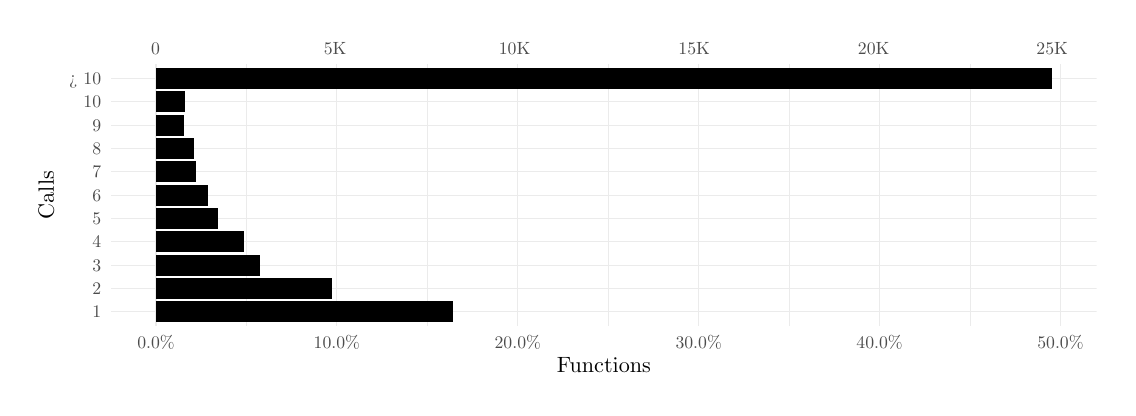
\begin{tikzpicture}[x=1pt,y=1pt]
\definecolor{fillColor}{RGB}{255,255,255}
\path[use as bounding box,fill=fillColor,fill opacity=0.00] (0,0) rectangle (390.26,130.09);
\begin{scope}
\path[clip] ( 30.17, 22.32) rectangle (386.26,116.83);
\definecolor{drawColor}{gray}{0.92}

\path[draw=drawColor,line width= 0.2pt,line join=round] ( 79.04, 22.32) --
	( 79.04,116.83);

\path[draw=drawColor,line width= 0.2pt,line join=round] (144.41, 22.32) --
	(144.41,116.83);

\path[draw=drawColor,line width= 0.2pt,line join=round] (209.77, 22.32) --
	(209.77,116.83);

\path[draw=drawColor,line width= 0.2pt,line join=round] (275.14, 22.32) --
	(275.14,116.83);

\path[draw=drawColor,line width= 0.2pt,line join=round] (340.51, 22.32) --
	(340.51,116.83);

\path[draw=drawColor,line width= 0.4pt,line join=round] ( 30.17, 27.38) --
	(386.26, 27.38);

\path[draw=drawColor,line width= 0.4pt,line join=round] ( 30.17, 35.82) --
	(386.26, 35.82);

\path[draw=drawColor,line width= 0.4pt,line join=round] ( 30.17, 44.26) --
	(386.26, 44.26);

\path[draw=drawColor,line width= 0.4pt,line join=round] ( 30.17, 52.70) --
	(386.26, 52.70);

\path[draw=drawColor,line width= 0.4pt,line join=round] ( 30.17, 61.14) --
	(386.26, 61.14);

\path[draw=drawColor,line width= 0.4pt,line join=round] ( 30.17, 69.58) --
	(386.26, 69.58);

\path[draw=drawColor,line width= 0.4pt,line join=round] ( 30.17, 78.01) --
	(386.26, 78.01);

\path[draw=drawColor,line width= 0.4pt,line join=round] ( 30.17, 86.45) --
	(386.26, 86.45);

\path[draw=drawColor,line width= 0.4pt,line join=round] ( 30.17, 94.89) --
	(386.26, 94.89);

\path[draw=drawColor,line width= 0.4pt,line join=round] ( 30.17,103.33) --
	(386.26,103.33);

\path[draw=drawColor,line width= 0.4pt,line join=round] ( 30.17,111.77) --
	(386.26,111.77);

\path[draw=drawColor,line width= 0.4pt,line join=round] ( 46.36, 22.32) --
	( 46.36,116.83);

\path[draw=drawColor,line width= 0.4pt,line join=round] (111.72, 22.32) --
	(111.72,116.83);

\path[draw=drawColor,line width= 0.4pt,line join=round] (177.09, 22.32) --
	(177.09,116.83);

\path[draw=drawColor,line width= 0.4pt,line join=round] (242.46, 22.32) --
	(242.46,116.83);

\path[draw=drawColor,line width= 0.4pt,line join=round] (307.82, 22.32) --
	(307.82,116.83);

\path[draw=drawColor,line width= 0.4pt,line join=round] (373.19, 22.32) --
	(373.19,116.83);
\definecolor{fillColor}{RGB}{0,0,0}

\path[fill=fillColor] ( 46.36,107.97) rectangle (370.07,115.57);

\path[fill=fillColor] ( 46.36, 23.58) rectangle (153.52, 31.18);

\path[fill=fillColor] ( 46.36, 99.53) rectangle ( 56.78,107.13);

\path[fill=fillColor] ( 46.36, 32.02) rectangle (109.88, 39.62);

\path[fill=fillColor] ( 46.36, 40.46) rectangle ( 83.98, 48.06);

\path[fill=fillColor] ( 46.36, 48.90) rectangle ( 78.12, 56.49);

\path[fill=fillColor] ( 46.36, 57.34) rectangle ( 68.81, 64.93);

\path[fill=fillColor] ( 46.36, 65.78) rectangle ( 65.03, 73.37);

\path[fill=fillColor] ( 46.36, 74.22) rectangle ( 60.74, 81.81);

\path[fill=fillColor] ( 46.36, 82.66) rectangle ( 60.20, 90.25);

\path[fill=fillColor] ( 46.36, 91.10) rectangle ( 56.47, 98.69);
\end{scope}
\begin{scope}
\path[clip] (  0.00,  0.00) rectangle (390.26,130.09);
\definecolor{drawColor}{gray}{0.30}

\node[text=drawColor,anchor=base,inner sep=0pt, outer sep=0pt, scale=  0.64] at ( 46.21,120.43) {0};

\node[text=drawColor,anchor=base,inner sep=0pt, outer sep=0pt, scale=  0.64] at (111.09,120.43) {5K};

\node[text=drawColor,anchor=base,inner sep=0pt, outer sep=0pt, scale=  0.64] at (175.96,120.43) {10K};

\node[text=drawColor,anchor=base,inner sep=0pt, outer sep=0pt, scale=  0.64] at (240.83,120.43) {15K};

\node[text=drawColor,anchor=base,inner sep=0pt, outer sep=0pt, scale=  0.64] at (305.70,120.43) {20K};

\node[text=drawColor,anchor=base,inner sep=0pt, outer sep=0pt, scale=  0.64] at (370.22,120.43) {25K};
\end{scope}
\begin{scope}
\path[clip] (  0.00,  0.00) rectangle (390.26,130.09);
\definecolor{drawColor}{gray}{0.30}

\node[text=drawColor,anchor=base east,inner sep=0pt, outer sep=0pt, scale=  0.64] at ( 26.57, 25.18) {1};

\node[text=drawColor,anchor=base east,inner sep=0pt, outer sep=0pt, scale=  0.64] at ( 26.57, 33.62) {2};

\node[text=drawColor,anchor=base east,inner sep=0pt, outer sep=0pt, scale=  0.64] at ( 26.57, 42.05) {3};

\node[text=drawColor,anchor=base east,inner sep=0pt, outer sep=0pt, scale=  0.64] at ( 26.57, 50.49) {4};

\node[text=drawColor,anchor=base east,inner sep=0pt, outer sep=0pt, scale=  0.64] at ( 26.57, 58.93) {5};

\node[text=drawColor,anchor=base east,inner sep=0pt, outer sep=0pt, scale=  0.64] at ( 26.57, 67.37) {6};

\node[text=drawColor,anchor=base east,inner sep=0pt, outer sep=0pt, scale=  0.64] at ( 26.57, 75.81) {7};

\node[text=drawColor,anchor=base east,inner sep=0pt, outer sep=0pt, scale=  0.64] at ( 26.57, 84.25) {8};

\node[text=drawColor,anchor=base east,inner sep=0pt, outer sep=0pt, scale=  0.64] at ( 26.57, 92.69) {9};

\node[text=drawColor,anchor=base east,inner sep=0pt, outer sep=0pt, scale=  0.64] at ( 26.57,101.13) {10};

\node[text=drawColor,anchor=base east,inner sep=0pt, outer sep=0pt, scale=  0.64] at ( 26.57,109.57) {> 10};
\end{scope}
\begin{scope}
\path[clip] (  0.00,  0.00) rectangle (390.26,130.09);
\definecolor{drawColor}{gray}{0.30}

\node[text=drawColor,anchor=base,inner sep=0pt, outer sep=0pt, scale=  0.64] at ( 46.36, 14.31) {0.0{\%}};

\node[text=drawColor,anchor=base,inner sep=0pt, outer sep=0pt, scale=  0.64] at (111.72, 14.31) {10.0{\%}};

\node[text=drawColor,anchor=base,inner sep=0pt, outer sep=0pt, scale=  0.64] at (177.09, 14.31) {20.0{\%}};

\node[text=drawColor,anchor=base,inner sep=0pt, outer sep=0pt, scale=  0.64] at (242.46, 14.31) {30.0{\%}};

\node[text=drawColor,anchor=base,inner sep=0pt, outer sep=0pt, scale=  0.64] at (307.82, 14.31) {40.0{\%}};

\node[text=drawColor,anchor=base,inner sep=0pt, outer sep=0pt, scale=  0.64] at (373.19, 14.31) {50.0{\%}};
\end{scope}
\begin{scope}
\path[clip] (  0.00,  0.00) rectangle (390.26,130.09);
\definecolor{drawColor}{RGB}{0,0,0}

\node[text=drawColor,anchor=base,inner sep=0pt, outer sep=0pt, scale=  0.80] at (208.22,  5.56) {Functions};
\end{scope}
\begin{scope}
\path[clip] (  0.00,  0.00) rectangle (390.26,130.09);
\definecolor{drawColor}{RGB}{0,0,0}

\node[text=drawColor,rotate= 90.00,anchor=base,inner sep=0pt, outer sep=0pt, scale=  0.80] at (  9.51, 69.58) {Calls};
\end{scope}
\end{tikzpicture}

  \caption{Call Distribution}
  \label{fig:callDist}
\end{figure}

We observe 294.45M arguments created in our execution traces. Of those 3.9M are
missing, 18.9M are $...$ arguments, and 271.6M are promises. These arguments
correspond to 185.9K parameter positions of the 50,435 functions for which we
generate signatures. Figure ~\ref{fig:paramDist} shows the distribution of these
parameters per function.

\begin{figure}[!h]
  \centering
  % Created by tikzDevice version 0.12.3.1 on 2021-04-09 22:35:57
% !TEX encoding = UTF-8 Unicode
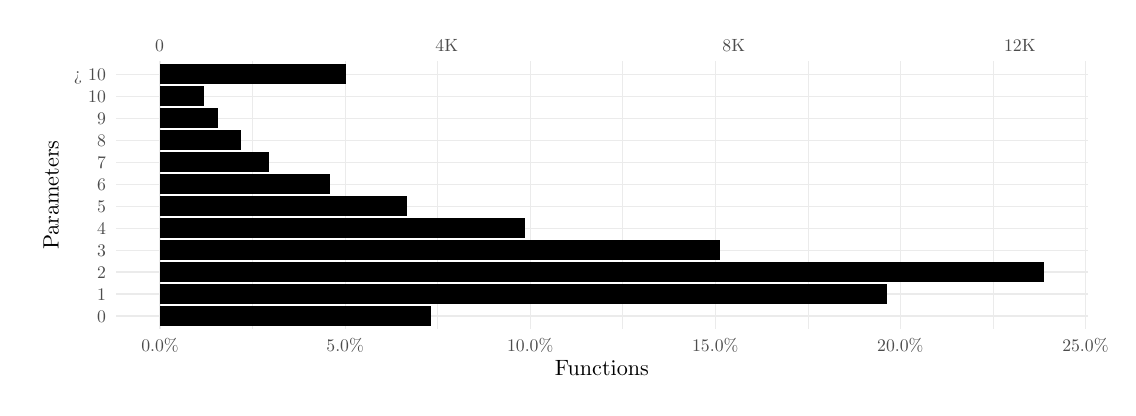
\begin{tikzpicture}[x=1pt,y=1pt]
\definecolor{fillColor}{RGB}{255,255,255}
\path[use as bounding box,fill=fillColor,fill opacity=0.00] (0,0) rectangle (390.26,130.09);
\begin{scope}
\path[clip] ( 31.86, 21.16) rectangle (383.14,117.99);
\definecolor{drawColor}{gray}{0.92}

\path[draw=drawColor,line width= 0.2pt,line join=round] ( 81.27, 21.16) --
	( 81.27,117.99);

\path[draw=drawColor,line width= 0.2pt,line join=round] (148.15, 21.16) --
	(148.15,117.99);

\path[draw=drawColor,line width= 0.2pt,line join=round] (215.02, 21.16) --
	(215.02,117.99);

\path[draw=drawColor,line width= 0.2pt,line join=round] (281.90, 21.16) --
	(281.90,117.99);

\path[draw=drawColor,line width= 0.2pt,line join=round] (348.77, 21.16) --
	(348.77,117.99);

\path[draw=drawColor,line width= 0.4pt,line join=round] ( 31.86, 25.92) --
	(383.14, 25.92);

\path[draw=drawColor,line width= 0.4pt,line join=round] ( 31.86, 33.86) --
	(383.14, 33.86);

\path[draw=drawColor,line width= 0.4pt,line join=round] ( 31.86, 41.80) --
	(383.14, 41.80);

\path[draw=drawColor,line width= 0.4pt,line join=round] ( 31.86, 49.73) --
	(383.14, 49.73);

\path[draw=drawColor,line width= 0.4pt,line join=round] ( 31.86, 57.67) --
	(383.14, 57.67);

\path[draw=drawColor,line width= 0.4pt,line join=round] ( 31.86, 65.61) --
	(383.14, 65.61);

\path[draw=drawColor,line width= 0.4pt,line join=round] ( 31.86, 73.54) --
	(383.14, 73.54);

\path[draw=drawColor,line width= 0.4pt,line join=round] ( 31.86, 81.48) --
	(383.14, 81.48);

\path[draw=drawColor,line width= 0.4pt,line join=round] ( 31.86, 89.42) --
	(383.14, 89.42);

\path[draw=drawColor,line width= 0.4pt,line join=round] ( 31.86, 97.35) --
	(383.14, 97.35);

\path[draw=drawColor,line width= 0.4pt,line join=round] ( 31.86,105.29) --
	(383.14,105.29);

\path[draw=drawColor,line width= 0.4pt,line join=round] ( 31.86,113.23) --
	(383.14,113.23);

\path[draw=drawColor,line width= 0.4pt,line join=round] ( 47.83, 21.16) --
	( 47.83,117.99);

\path[draw=drawColor,line width= 0.4pt,line join=round] (114.71, 21.16) --
	(114.71,117.99);

\path[draw=drawColor,line width= 0.4pt,line join=round] (181.58, 21.16) --
	(181.58,117.99);

\path[draw=drawColor,line width= 0.4pt,line join=round] (248.46, 21.16) --
	(248.46,117.99);

\path[draw=drawColor,line width= 0.4pt,line join=round] (315.34, 21.16) --
	(315.34,117.99);

\path[draw=drawColor,line width= 0.4pt,line join=round] (382.21, 21.16) --
	(382.21,117.99);
\definecolor{fillColor}{RGB}{0,0,0}

\path[fill=fillColor] ( 47.83,109.66) rectangle (115.04,116.80);

\path[fill=fillColor] ( 47.83, 22.35) rectangle (145.68, 29.50);

\path[fill=fillColor] ( 47.83, 30.29) rectangle (310.59, 37.43);

\path[fill=fillColor] ( 47.83,101.72) rectangle ( 63.63,108.86);

\path[fill=fillColor] ( 47.83, 38.23) rectangle (367.18, 45.37);

\path[fill=fillColor] ( 47.83, 46.16) rectangle (250.08, 53.31);

\path[fill=fillColor] ( 47.83, 54.10) rectangle (179.66, 61.24);

\path[fill=fillColor] ( 47.83, 62.04) rectangle (137.11, 69.18);

\path[fill=fillColor] ( 47.83, 69.97) rectangle (109.42, 77.12);

\path[fill=fillColor] ( 47.83, 77.91) rectangle ( 87.10, 85.05);

\path[fill=fillColor] ( 47.83, 85.85) rectangle ( 77.25, 92.99);

\path[fill=fillColor] ( 47.83, 93.78) rectangle ( 68.76,100.93);
\end{scope}
\begin{scope}
\path[clip] (  0.00,  0.00) rectangle (390.26,130.09);
\definecolor{drawColor}{gray}{0.30}

\node[text=drawColor,anchor=base,inner sep=0pt, outer sep=0pt, scale=  0.64] at ( 47.69,121.59) {0};

\node[text=drawColor,anchor=base,inner sep=0pt, outer sep=0pt, scale=  0.64] at (151.42,121.59) {4K};

\node[text=drawColor,anchor=base,inner sep=0pt, outer sep=0pt, scale=  0.64] at (255.15,121.59) {8K};

\node[text=drawColor,anchor=base,inner sep=0pt, outer sep=0pt, scale=  0.64] at (358.53,121.59) {12K};
\end{scope}
\begin{scope}
\path[clip] (  0.00,  0.00) rectangle (390.26,130.09);
\definecolor{drawColor}{gray}{0.30}

\node[text=drawColor,anchor=base east,inner sep=0pt, outer sep=0pt, scale=  0.64] at ( 28.26, 23.72) {0};

\node[text=drawColor,anchor=base east,inner sep=0pt, outer sep=0pt, scale=  0.64] at ( 28.26, 31.66) {1};

\node[text=drawColor,anchor=base east,inner sep=0pt, outer sep=0pt, scale=  0.64] at ( 28.26, 39.59) {2};

\node[text=drawColor,anchor=base east,inner sep=0pt, outer sep=0pt, scale=  0.64] at ( 28.26, 47.53) {3};

\node[text=drawColor,anchor=base east,inner sep=0pt, outer sep=0pt, scale=  0.64] at ( 28.26, 55.47) {4};

\node[text=drawColor,anchor=base east,inner sep=0pt, outer sep=0pt, scale=  0.64] at ( 28.26, 63.40) {5};

\node[text=drawColor,anchor=base east,inner sep=0pt, outer sep=0pt, scale=  0.64] at ( 28.26, 71.34) {6};

\node[text=drawColor,anchor=base east,inner sep=0pt, outer sep=0pt, scale=  0.64] at ( 28.26, 79.28) {7};

\node[text=drawColor,anchor=base east,inner sep=0pt, outer sep=0pt, scale=  0.64] at ( 28.26, 87.21) {8};

\node[text=drawColor,anchor=base east,inner sep=0pt, outer sep=0pt, scale=  0.64] at ( 28.26, 95.15) {9};

\node[text=drawColor,anchor=base east,inner sep=0pt, outer sep=0pt, scale=  0.64] at ( 28.26,103.09) {10};

\node[text=drawColor,anchor=base east,inner sep=0pt, outer sep=0pt, scale=  0.64] at ( 28.26,111.02) {> 10};
\end{scope}
\begin{scope}
\path[clip] (  0.00,  0.00) rectangle (390.26,130.09);
\definecolor{drawColor}{gray}{0.30}

\node[text=drawColor,anchor=base,inner sep=0pt, outer sep=0pt, scale=  0.64] at ( 47.83, 13.15) {0.0{\%}};

\node[text=drawColor,anchor=base,inner sep=0pt, outer sep=0pt, scale=  0.64] at (114.71, 13.15) {5.0{\%}};

\node[text=drawColor,anchor=base,inner sep=0pt, outer sep=0pt, scale=  0.64] at (181.58, 13.15) {10.0{\%}};

\node[text=drawColor,anchor=base,inner sep=0pt, outer sep=0pt, scale=  0.64] at (248.46, 13.15) {15.0{\%}};

\node[text=drawColor,anchor=base,inner sep=0pt, outer sep=0pt, scale=  0.64] at (315.34, 13.15) {20.0{\%}};

\node[text=drawColor,anchor=base,inner sep=0pt, outer sep=0pt, scale=  0.64] at (382.21, 13.15) {25.0{\%}};
\end{scope}
\begin{scope}
\path[clip] (  0.00,  0.00) rectangle (390.26,130.09);
\definecolor{drawColor}{RGB}{0,0,0}

\node[text=drawColor,anchor=base,inner sep=0pt, outer sep=0pt, scale=  0.80] at (207.50,  4.40) {Functions};
\end{scope}
\begin{scope}
\path[clip] (  0.00,  0.00) rectangle (390.26,130.09);
\definecolor{drawColor}{RGB}{0,0,0}

\node[text=drawColor,rotate= 90.00,anchor=base,inner sep=0pt, outer sep=0pt, scale=  0.80] at ( 11.20, 69.58) {Parameters};
\end{scope}
\end{tikzpicture}

  \caption{Parameter Distribution}
  \label{fig:paramDist}
\end{figure}

7.3\% functions have 0 parameters, 19.6\% have 1, and 5.0\% have over 10. There
are 15 functions with over 50 parameters that come from 10 packages.
\c{ComplexHeatmap::pheatmap} (51), \c{network::plot.network.default} (52),
\c{rpart.plot::get.layout} (53), \c{sna::gplot} (54), \c{Hmisc::latex.default}
(55), \c{VennDiagram::draw.quintuple.venn} (57) \c{pROC::plot.roc.roc} (58),
\c{rpart.plot::draw.node.numbers} (60), \c{gplots::heatmap.2} (63),
\c{Hmisc::event.chart} (66), \c{ComplexHeatmap::Heatmap} (83),
\c{ggplot2::theme} (95), \c{ergm::control.ergm} (117), \c{rpart.plot::prp}
(119), and \c{rpart.plot::check.if.dot.arg.supported.by.rpart.rules} (122) with
the highest number of parameters.

Now, we turn our attention to the algorithm used by \lazr to infer strictness.
As discussed in section \ref{subsection:lazr}, \lazr uses execution traces to
synthesize strictness signatures. Execution traces tell us if an argument
\emph{(a)} is evaluated, \emph{(b)} is passed to a $...$ parameter, \emph{(c)}
is metaprogrammed, \emph{(d)} performs a non-local effect, and \emph{(e)}
accesses parent environment reflectively. \lazr merges this information from all
execution traces to get a summary of operations for a function parameter
position. It uses this summary decide if an argument can be evaluated eagerly
and generates strictness signatures. The signatures also dictate the order of
evaluation of arguments.

Because of the difficulty in assigning a unique strictness signature, $...$
arguments are always lazy. Meta-programmed arguments are also lazy as
meta-programming relies on unevaluated argument text provided by a promise. The
remaining operations are sources of \emph{accidental laziness}. We could decide
to unevaluated, effectful, and reflective arguments lazy to preserve the
semantics of legacy code. Or, we could make them strict to get rid of more
promises at the risk of breaking code. The impact of this choice is not clear
upfront. Hence, \lazr synthesizes multiple strictness signature
``configurations`` to facilitate this assessment. It is worth noting that making
arguments lazy if they are side-effecting has the potential to make everything
lazy because it is dependent on how a client invokes the API. \lazr only makes
the parameter lazy if an argument has performed a side-effect or reflective
operation in the programs it has run. Including more programs will make more
arguments lazy.

Now, we take a detailed look at the different sources of laziness.

There are XXXX $...$ parameters. We unconditionally treat them lazy.

\subsubsection{Metaprogramming}
For tracking metaprogramming, we look at uses of \code{substitute} on arguments
from R code and \code{PREXPR} macro on promise objects from C code. We observe
substitute called on XXX arguments from XXXX parameters of XXXX functions.
\code{PREXPR} was called on XXX arguments from XXXX parameters of XXXX
functions.

For an in-depth discussion on the patterns of use of \code{substitute}, we refer
the reader to \citet{oopsla19b}. We continue with the exploration of the use of
\code{PREXPR} for metaprogramming, since that is not addressed in
\cite{oopsla19b}.

We observe that 




\subsubsection{Unevaluated Arguments}
Of the 294.45M total arguments in our corpus, 30.4M argument promises were not
evaluated. They correspond to 52,083 parameters of 26,398 functions from 473
packages. These functions are non-strict in the corresponding parameters.

Based on argument evaluation, we can classify parameter positions into three
categories.\always parameters are those whose arguments are evaluated in all
calls. \sometimes parameters are those whose arguments are evaluated at least
once but not always. \never parameters are those whose arguments are never
evaluated. Table~\ref{table:argeval} shows the number and proportion of
parameters that belong to these categories.

\begin{table}[!h]
  \vspace{-3mm}
  \caption{Argument Evaluation}\label{table:argeval}
  \vspace{-3mm}
  \begin{tabular}{lr|lr|lr}
    \toprule
    \textbf{Type}&\multicolumn{2}{c}{\textbf{Parameters}}&\multicolumn{2}{c}{\textbf{Functions}}&\textbf{Packages}\\
    \midrule
    Always&144565&73.51\%&48456&96.08\%&490\\
    Sometimes&16411&8.35\%&7070&14.02\%&410\\
    Never&10637&5.41\%&5907&11.71\%&405\\
    \midrule
    Sometimes*&15130&7.69\%&6609&13.1\%&406\\
    Never*&9251&4.7\%&5121&10.15\%&400\\
    \bottomrule
  \end{tabular}
\end{table}

Majority of parameters are \always parameters, suggesting that arguments passed
to functions are evaluated in most of the cases. This is followed by 8.35\%
\sometimes parameters. Their presence indicates use of metaprogramming or
unexplored control flow paths in the function. Lastly, we have 5.41\% \never
arguments whose presence indicates lack of coverage, metaprogramming, or dummy
parameter. The \textbf{Functions} field gives the number of functions with
\always, \sometimes, and \never arguments. The same function can appear in
multiple columns since different parameters can have different evaluation
classification. The \textbf{Packages} field of Table~\ref{table:areval} tells us
that \never and \sometimes functions are spread across many packages.


\sometimesStar and \neverStar in Table~\ref{table:argeval} are the number of
\sometimes and \never cases without metaprogrammed. The different is small which
suggests that metaprogramming is not the primary reason for arguments remaining
unevaluated. Turning to the number of calls, we find that 78.33\% of functions
with \never parameters are called more than once. This suggests that a lack of
call diversity could be one of factors for \never arguments' existence. With
better call diversity, the \never parameters will turn into \sometimes.

\paragraph{Qualitative Analysis}

We analyzed a sample of functions with \sometimes and \never parameters to
identify usage patterns.

First, we look at \sometimes parameters. A common patter occurring in 30
packages is the following definition of \code{\%||\%} function.

\begin{lstlisting}
lazyeval::\%||\% <- function(x, y) if(is.null(x)) y else x
\end{lstlisting}

This function evaluates its second argument \code{y} only if \code{x} is
\code{NULL}. This makes \code{y} a \sometimes parameter. This pattern suggests
that \code{y} is a \sometimes parameter for a reason and should not be evaluated
unless needed. However, there are other functions with multiple paths where
evaluating the \sometimes argument is expected to be benign. For example, in
\code{bayesplot::is_whole_number} function, the \code{tol} argument is only
evaluated when \code{x} is a numeric value. I

\begin{lstlisting}
bayesplot::is_whole_number <- function(x, tol = .Machine$double.eps) {
    if (!is.numeric(x)) { FALSE } else { abs(x - round(x)) < tol }
}
\end{lstlisting}


Another pattern occurring in 4 packages is the definition of
\code{on_package_load}.

\begin{lstlisting}
glue::on_package_load <- function(pkg, expr) {
    if (isNamespaceLoaded(pkg)) { expr }
    else {
        thunk <- function(...) expr
        setHook(packageEvent(pkg, "onLoad"), thunk)
    }
}
\end{lstlisting}

Here, if package \code{pkg} is not loaded, the \code{expr} argument's evaluation
is delayed until the package's \code{onLoad} event occurs. In some executions,
we see the \code{expr} argument being evaluated if package \code{pkg} is loaded
and in other iterations, we don't. The way this code is written suggests that
\code{expr} should not be evaluated strictly.

S3 generics result in many \sometimes and \never parameters. These functions
dynamically dispatch to a specific implementation with the same name based on
the first argument's class. In this case, the first argument is always evaluated
but the remaining arguments might not be needed by the specific method. Across
all executions, we observed that \code{n} and \code{m} are evaluated sometimes
but \code{r} is never evaluated.

\begin{lstlisting}
abind::acorn <- function(x, n=6, m=5, r=1, ...) UseMethod('acorn')
\end{lstlisting}


Next, we turn our attention to \never parameters.

The most common case is when an argument is not used in some branch of the
function. Due to lack of call diversity, the branch in which the argument is
used is never taken and the parameter is classified as \never. For example,
\code{discretize} function of package \code{actuar} only uses \code{xlim} if
\code{from} and \code{to} parameters are missing.
\begin{lstlisting}
actuar:::discretize <- function (cdf, from, to, ..., xlim = NULL) {
    ...
    if (missing(from)) from <- xlim[1];
    if (missing(to)) to <- xlim[2];
    ...
}
\end{lstlisting}


Another pattern leading to \never parameters is when a function is called with a
certain interface even if it does not use those arguments. R calls a package's
\code{.onLoad} function with arguments \code{libname} and \code{pkgname} when
the package is loaded. The \code{.onLoad} hook of \code{assertive.base} package
ignores them.
\begin{lstlisting}
assertive.base::.onLoad <- function(libname, pkgname) {
    options(assertive.severity = "stop")
}
\end{lstlisting}

The \code{proxy} package defines over a dozen methods with the interface
\code{function(a, b, c, d, n) ...} that implement different proximity metrics by
using only a subset of the arguments.
This also happens in method dispatch when the generic method defines a parameter
which is not used by the specific method. For example \code{bit64} package
defines \code{unipos} generic method with a parameter \code{incomparables} which
is not used by its only concrete implementation \code{unipos.integer64}


Sometimes arguments don't need to be used by design.
The \code{tail} operation in package \code{dbplyr} is not defined for
\code{tbl_lazy} objects. So the function throws an error when called without
using any of its arguments.
\begin{lstlisting}
dbplyr::tail.tbl_lazy <- function(x, n = 6L, ...) {
    stop("tail() is not supported by sql sources", call. = FALSE)
}
\end{lstlisting}

Sometimes packages implement a specialized compatible wrapper.
\code{jsonlite} package implements \code{stop} function with the same interface
as R's \code{base} package's \code{stop} function but ignores its \code{call.}
argument.
\begin{lstlisting}
jsonlite::stop <- function(..., call. = FALSE) {
    base::stop(..., call. = FALSE)
}
\end{lstlisting}

\never parameters can also represent an erroneous condition that would not
happen in a correct program. In \code{codetools} package, function
\code{checkSymOrString} fails if the argument does not have the correct type. In
all the calls we observed, the \code{signal} argument was not used because
\code{e} had the correct type.
\begin{lstlisting}
codetools::checkSymOrString <- function(e, signal = stop) {
    type <- typeof(e)
    if (type == "symbol" || type == "character") e
    else signal("not a symbol or string")
}
\end{lstlisting}

\subsubsection{Reflection}

R allows reflective access to parent scope through \code{as.environment} and
\code{pos.to.env} functions when called with argument \code{-1}.
They return the environment of the caller with respect to call in which they are

evaluated. Consider the following example in which function f is called with the
same argument \code{as.environment(-1)} for both \code{x} and \code{y}
parameters. The first argument \code{x} is evaluated immediately inside
function \code{f} and the second argument \code{y} is evaluated inside the
\code{id} function. \code{x} evaluates to the environment of the parent of
\code{f} which is the \code{global} environment, whereas \code{y} evaluates to
the environment of \code{f} which is the parent of \code{id} inside of which
\code{y} is evaluated.

\begin{lstlisting}
id <- function(a) a
f <- function(x, y) { x; id(y); }
f(x = as.environment(-1), y = as.environment(-1))
\end{lstlisting}

There are two points to note here. First, the strictness of \code{f} with
respect to \code{x} and \code{y} depends on how \code{f} is called. Second,
\code{f} will now be lazy in argument \code{y}, otherwise we will end up
evaluating inside \code{f}. Erroneously evaluating \code{y} strictly would
result in an incorrect environment, but not an error, which could turn into a
debugging nightmare.

\code{as.environment} is internally implemented using \code{pos.to.env} so the
two functions have same semantics when called with \code{-1} as the argument.

It is interesting to note that there are other functions providing reflective
access to call stack frames such as \code{parent.frame}, \code{sys.frame}, etc.
However, these take into account the current evaluation environment to identify
the parent caller. A promise evaluates the argument expression inside the
caller's environment. So, a call to \code{parent.frame()} directly inside the
argument will use the caller's environment to identify the parent dynamic scope.
This makes its result independent of the point at which the promise is
evaluated.

Another wrinkle introduced by this setup is that it can transitively affect the
strictness of other function arguments. Imagine \code{f} is called from \code{g}
as shown below.

\begin{lstlisting}
g <- function(u, v) {
    f(u, v)
}
g(as.environment(-1), as.environment(-1))
\end{lstlisting}

Clearly, in this case we have to make \code{g} non-strict in \code{u} and
\code{v}. Their results depend upon how they are evaluated inside \code{f}.

We identified 2710 arguments which directly call \code{as.environment(-1)} and
\code{pos.to.env(-1)} in our corpus. They correspond to 2 parameters from 2
functions, \code{R.oo::.getFunctionByName}, and \code{backports:::get0}.

\code{R.oo:::.getFunctionByName} is a private function of \code{R.oo} package
which searches for a function by name in different scopes, configured by its
arguments. Its fourth parameter, \code{callEnvir}, has a default value of
\code{as.environment(-1)}. It is called 2707 times. The relevant part of its
definition is that \code{callEnvir} is evaluated by assigning it to
\code{envirT} before it is passed down to the \code{exists} function.

\begin{lstlisting}
function(name, where = c("ns", "search", "ns*"),
         envir = NULL, callEnvir = as.environment(-1L),
         class = "function", mustExist = TRUE, ...) {
    ...
    envirT <- callEnvir
    if (exists(name, mode = "function", envir = envirT, inherits = TRUE))
    ...
}
\end{lstlisting}

\code{backports::get0} is a private function of \code{backports} package which
looks up a variable in a scope, similar in spirit to
\code{R.oo:::.getFunctionByName}. This function is called 3 times, always with
the default value \code{pos.to.env(-1)} for \code{envir} argument. Unlike
\code{R.oo:::.getFunctionByName}, \code{backports:::get0} passes \code{envir}
unevaluated to \code{mget}. \code{mget} in turn evaluates \code{envir} and looks
up variable referred to by \code{x} in \code{envir}. Clearly, with the default
value of \code{envir}, lookup will happen in the environment of
\code{backports::get0} which only has bindings for its parameters. What makes
this work is that it is only called from the top-level, with the argument
\code{inherits} set to \code{TRUE}. This causes \code{mget} to search
recursively in enclosing scopes beginning from \code{envir} until lookup
succeeds in the \code{global} environment used for top-level bindings.

\begin{lstlisting}
function (x, envir = pos.to.env(-1L), mode = "any",
          inherits = TRUE, ifnotfound = NULL)  {
    ....
    mget(x[1L], envir = envir, mode = mode,
         inherits = inherits, ifnotfound = list(ifnotfound))[[1L]]
}
\end{lstlisting}

Calls to \code{R.oo:::.getFunctionByName} result in transitively making 1821
argument lazy. They correspond to 18 parameters from 15 functions of 3 packages.
We manually analyzed these cases but found that none of these functions pass
their arguments containing calls to \code{as.environment(-1)} or
\code{pos.to.env(-1)} to \code{R.oo:::.getFunctionByName}. They are identified
as lazy because our dynamic analyzer is conservative. When a reflective call
happens from an argument promise, it taints all the function arguments on the
stack. This has the effect of making more arguments lazy than needed.

\code{backports::get0} is invoked from the top-level so it does not result in
spurious transitive laziness.

\subsubsection{Side-Effects}

\begin{table}
  \vspace{-3mm}
  \small
  \caption{Effects} \label{table:effects}
  \centering
  \begin{tabular}{lllll}
    \toprule
    \textbf{Effect}&\textbf{Count}&\textbf{Parameters}&\textbf{Functions}&\textbf{Packages}\\
    \midrule
    L&3739631&5539&3619&358\\
    D&1069746&2972&2599&319\\
    A&236985&510&486&109\\
    R&1172&27&24&10\\
    E&6&6&6&3\\
    \bottomrule
  \end{tabular}
\end{table}

\begin{table}
  \vspace{-3mm}
  \small
  \caption{Effect Sequence} \label{table:effectseq}
  \centering
  \begin{tabular}{lll}
    \toprule
    \textbf{Effect Sequence}&\textbf{Argument \%}\\
    \midrule
    (L+D+)+&40.35\%\\
    L+&29.75\%\\
    D+&10.25\%\\
    (L+A+)+&6.96\%\\
    (D+A+)+D+&3.23\%\\
    A+&2.48\%\\
    (L+D+)+L+&1.69\%\\
    (D+A+)+&1.42\%\\
    (L+D+)+(L+A+)+(L+D+)+&0.99\%\\
    (L+D+)+A+&0.5\%\\
    \bottomrule
  \end{tabular}
\end{table}

\subsection{Summary}

Table~\ref{table:strictdist} presents a summary of the distribution of
parameters, functions, and packages that correspond to unevaluated, effectful or
reflective arguments. Row \#0 tells that there are 128.3K parameters from 44.4K
functions whose arguments are evaluated across all calls and they don't perform
any effect or reflective operation. Similarly, row \#7 tells us that 25
parameters from 24 functions are not evaluated in at least one call, but whey
they are evaluated, they perform a side-effect and a reflective operation.
Similarly, row \#4 tells us that 27.1K parameters from 11.3K functions are never
evaluated. A careful study of these rows yields the following insights. First,
arguments passed to majority of parameters, 65.25\%, are always evaluated and
don't perform any side-effects or reflective operations. So, they can be made
unconditionally strict . Of the remaining parameters, only unevaluated arguments
correspond to 13.76\% parameters, followed by only side-effecting arguments to
4\% parameters, and only reflective promises to 0.07\% parameters. The remaining
combinations amount to less than a percent each. It is important to note that a
function can appear in multiple rows as different parameters can belong to
different categories. Same reasoning applies to packages. Another interesting
pattern in the data is that arguments performing reflective operations
(alternate rows \#1, \#3, \#5, \#7) come from relatively few functions and
packages.

\begin{table}
  \vspace{-3mm}
  \small
  \caption{Strictness Distribution} \label{table:strictdist}
  \centering
  \begin{tabular}{lcccr|lr|lr}
    \toprule
    \#&\bf Unevaluted & \bf Side-Effecting & \bf Reflective & \multicolumn{2}{c}{\textbf{Parameters}} & \multicolumn{2}{c}{\textbf{Functions}}& \bf Packages\\
    \midrule
    0&\xmark{}&\xmark{}&\xmark{}&128305&65.25\%&44377&85.93\%&489\\
    1&\xmark{}&\xmark{}&\cmark{}&134&0.07\%&124&0.24\%&47\\
    2&\xmark{}&\cmark{}&\xmark{}&7871&4\%&5805&11.24\%&399\\
    3&\xmark{}&\cmark{}&\cmark{}&408&0.21\%&385&0.75\%&93\\
    4&\cmark{}&\xmark{}&\xmark{}&27050&13.76\%&11333&21.95\%&453\\
    5&\cmark{}&\xmark{}&\cmark{}&13&0.01\%&12&0.02\%&11\\
    6&\cmark{}&\cmark{}&\xmark{}&1213&0.62\%&813&1.57\%&199\\
    7&\cmark{}&\cmark{}&\cmark{}&25&0.01\%&24&0.05\%&15\\
    \bottomrule
  \end{tabular}
\end{table}

An important detail in this summary is that includes contribution of
side-effects and reflective operations performed by R's \emph{base} package and
other user packages not part of our corpus. This is because arguments are also
transitively involved in side-effecting or reflective operations. The numbers
provided in this table are upper-bounds, we over count the number of arguments
transitively involved in effects and reflective operations because our inference
algorithm is conservative.

\subsection{Orders of Evaluation}

The argument evaluation orders observed for a function depend on its
implementation and the control-flow paths exercised by its inputs. In this work
we ignore this evaluation order. For evaluation robustness, we choose the
definition order in the synthesized signatures. For assessing performance, the
\Rsh just-in-time compiler uses the call order, i.e., the order in which
arguments are passed to the function at the call site.

Our notion of strictness departs from that of ~\citet{oopsla19b}. According to
them, a function is strict if it evaluates all of its argument in a single
pre-ordained order.

\AG{add evaluation orders and contrast with side effects to assess impact.}
%%the function and choose the definition order.
%%Figure~\ref{fig:force_order} shows the number of evaluation orders of the
%%functions in our corpus. XX(XX\%) functions have a single evaluation order. Out
%%of those, XX functions evaluate all of their arguments. Evaluation orders
%%greater than 5 are rare and are found only in XX functions.


\section{Compile the Lazy Away}

In this section we report on our experiments to evaluate the implications of
eagerness on an implementations of R. To that end we modified \Rsh, a just-in-time
compiler for the language. \Rsh is based on the GNU R reference implementation
and introduces an additional two-tiered compilation strategy. The
first tier is realized by a naive bytecode interpreter, the second tier
by an optimizing native compiler. The compiler employs, among many other
optimizations, speculative inlining of R closures and promises \citep{dls19,
oopsla20c}.
The reason for choosing \Rsh as the target for our
experiments is, that it allows us to better evaluate the impact of lazyness. In
\Rsh we can both measure the impact on an interpreter with few optimizations
applied to the bytecode and an optimizing compiler, that already does its best
eliding promises as long as the default semantics allow it.
To conduct our evaluation, we changed the first-tier
compiler to eagerly evaluate all arguments at all call-sites, except for a
manually curated list of exceptions.
In the following we will refer
to this modified implementation as \Rshstrict.

Our main hypothesis regarding performance is that eager semantics lead to faster
execution of R programs. This hypothesis might seem unexpected to some readers,
as call-by-need is sometimes used to avoid unnecessary computation in a program.
On the other hand, delaying computations is more complex to implement and we
observed it to obstruct performance in two ways: First, it leads to more
allocations of promises used to represent the delayed computation. Second, in
combination with effects potentially originating from promises, it obstructs
more advanced compiler analysis and optimizations. Especially the later point
means that we expect the hypothesis to hold even for a just-in-time compiler,
that uses advanced optimizations.
In particular, we pose the following predictions:
(1) eager semantics should improve performance of most benchmarks for both tiers
of \Rsh; (2) a significant portion of the speedup is due to reduced garbage
collection pressure; (3) and there is an additional speedup due to improved compiler
optimizations. In the following we will present our evidence in support of all
three predictions.

We evaluate the effects of our modifications on the Ř benchmark suite.
To ease the discussion, the results are presented on a representative subset of
the suite which includes one variant of
each benchmark. As should be no surprise given the results presented so far,
only a handful of functions, such as
\lstinline{tryCatch} had to be kept lazy for all the benchmarks to compute
the correct results.

\paragraph{Methodology}

All of the following experiments are run on a dedicated benchmark machine, with
all background tasks disabled. The system features an Intel i7-6700K CPU, stepping 3,
microcode 0xe2 with 4 cores and 8 threads. The system has 32 GB of RAM and is
running Ubuntu 18.04 on a 4.15.0-136 Linux kernel. For ease of use, experiments
are built as OCI compliant containers, based on Ubuntu 20.04, and executed on
the Docker runtime 20.10.5, build 55c4c88. We verified the overhead introduced by
the containerization to be uniform. All measurements are taken repeatedly and we
keep a historical record to spot instable behavior. This lead us to exclude the
\lstinline{convolution} benchmark from the suite, which appears to have a
bi-modal performance profile, likely caused by the llvm backend of \Rsh.

Performance measurements are gathered by running $t_e$ invocations of \Rsh on
each benchmark. Within each invocation we measure the execution time of $t_i$
in-process invocations. For each invocation the first 5 in-process iterations
are discarded, to exclude warmup behavior. Agregate numbers are reported as the
speedup over the arithmetic mean of the execution times. Multiple speedup
numbers are averaged with a geometric mean. To establish a baseline we measured
the speedup of \Rsh over GNU R, on our selection of the benchmark suite with
$t_e = 1, t_i = 15$ and found a mean speedup of \speedupRsh, ranging between
\speedupRshMin and \speedupRshMax.

\paragraph{Speedup}

\begin{figure}[h]
  \centering
  % Created by tikzDevice version 0.12.3.1 on 2021-04-16 11:39:57
% !TEX encoding = UTF-8 Unicode
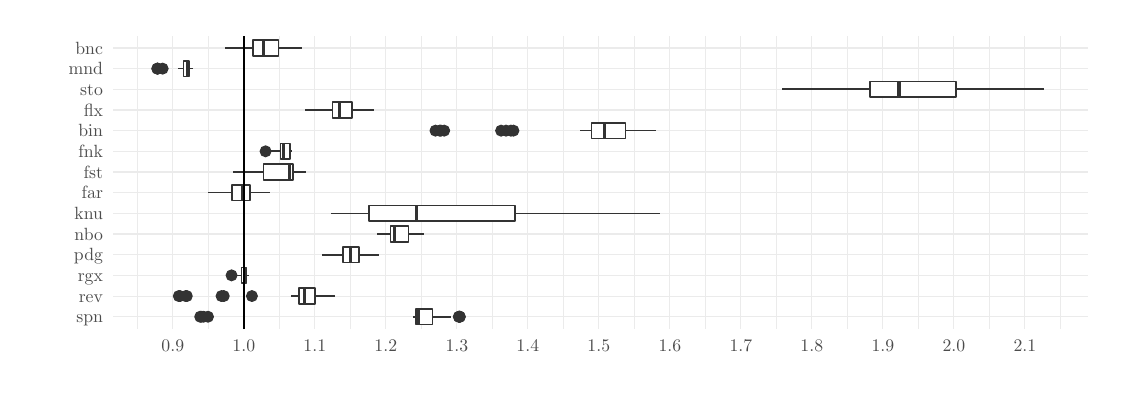
\begin{tikzpicture}[x=1pt,y=1pt]
\definecolor{fillColor}{RGB}{255,255,255}
\path[use as bounding box,fill=fillColor,fill opacity=0.00] (0,0) rectangle (390.26,130.09);
\begin{scope}
\path[clip] ( 30.80, 21.16) rectangle (383.14,127.24);
\definecolor{drawColor}{gray}{0.92}

\path[draw=drawColor,line width= 0.2pt,line join=round] ( 39.61, 21.16) --
	( 39.61,127.24);

\path[draw=drawColor,line width= 0.2pt,line join=round] ( 65.27, 21.16) --
	( 65.27,127.24);

\path[draw=drawColor,line width= 0.2pt,line join=round] ( 90.93, 21.16) --
	( 90.93,127.24);

\path[draw=drawColor,line width= 0.2pt,line join=round] (116.58, 21.16) --
	(116.58,127.24);

\path[draw=drawColor,line width= 0.2pt,line join=round] (142.24, 21.16) --
	(142.24,127.24);

\path[draw=drawColor,line width= 0.2pt,line join=round] (167.90, 21.16) --
	(167.90,127.24);

\path[draw=drawColor,line width= 0.2pt,line join=round] (193.55, 21.16) --
	(193.55,127.24);

\path[draw=drawColor,line width= 0.2pt,line join=round] (219.21, 21.16) --
	(219.21,127.24);

\path[draw=drawColor,line width= 0.2pt,line join=round] (244.87, 21.16) --
	(244.87,127.24);

\path[draw=drawColor,line width= 0.2pt,line join=round] (270.52, 21.16) --
	(270.52,127.24);

\path[draw=drawColor,line width= 0.2pt,line join=round] (296.18, 21.16) --
	(296.18,127.24);

\path[draw=drawColor,line width= 0.2pt,line join=round] (321.84, 21.16) --
	(321.84,127.24);

\path[draw=drawColor,line width= 0.2pt,line join=round] (347.50, 21.16) --
	(347.50,127.24);

\path[draw=drawColor,line width= 0.2pt,line join=round] (373.15, 21.16) --
	(373.15,127.24);

\path[draw=drawColor,line width= 0.4pt,line join=round] ( 30.80, 25.64) --
	(383.14, 25.64);

\path[draw=drawColor,line width= 0.4pt,line join=round] ( 30.80, 33.11) --
	(383.14, 33.11);

\path[draw=drawColor,line width= 0.4pt,line join=round] ( 30.80, 40.59) --
	(383.14, 40.59);

\path[draw=drawColor,line width= 0.4pt,line join=round] ( 30.80, 48.06) --
	(383.14, 48.06);

\path[draw=drawColor,line width= 0.4pt,line join=round] ( 30.80, 55.53) --
	(383.14, 55.53);

\path[draw=drawColor,line width= 0.4pt,line join=round] ( 30.80, 63.00) --
	(383.14, 63.00);

\path[draw=drawColor,line width= 0.4pt,line join=round] ( 30.80, 70.47) --
	(383.14, 70.47);

\path[draw=drawColor,line width= 0.4pt,line join=round] ( 30.80, 77.94) --
	(383.14, 77.94);

\path[draw=drawColor,line width= 0.4pt,line join=round] ( 30.80, 85.41) --
	(383.14, 85.41);

\path[draw=drawColor,line width= 0.4pt,line join=round] ( 30.80, 92.88) --
	(383.14, 92.88);

\path[draw=drawColor,line width= 0.4pt,line join=round] ( 30.80,100.35) --
	(383.14,100.35);

\path[draw=drawColor,line width= 0.4pt,line join=round] ( 30.80,107.82) --
	(383.14,107.82);

\path[draw=drawColor,line width= 0.4pt,line join=round] ( 30.80,115.29) --
	(383.14,115.29);

\path[draw=drawColor,line width= 0.4pt,line join=round] ( 30.80,122.76) --
	(383.14,122.76);

\path[draw=drawColor,line width= 0.4pt,line join=round] ( 52.44, 21.16) --
	( 52.44,127.24);

\path[draw=drawColor,line width= 0.4pt,line join=round] ( 78.10, 21.16) --
	( 78.10,127.24);

\path[draw=drawColor,line width= 0.4pt,line join=round] (103.75, 21.16) --
	(103.75,127.24);

\path[draw=drawColor,line width= 0.4pt,line join=round] (129.41, 21.16) --
	(129.41,127.24);

\path[draw=drawColor,line width= 0.4pt,line join=round] (155.07, 21.16) --
	(155.07,127.24);

\path[draw=drawColor,line width= 0.4pt,line join=round] (180.72, 21.16) --
	(180.72,127.24);

\path[draw=drawColor,line width= 0.4pt,line join=round] (206.38, 21.16) --
	(206.38,127.24);

\path[draw=drawColor,line width= 0.4pt,line join=round] (232.04, 21.16) --
	(232.04,127.24);

\path[draw=drawColor,line width= 0.4pt,line join=round] (257.70, 21.16) --
	(257.70,127.24);

\path[draw=drawColor,line width= 0.4pt,line join=round] (283.35, 21.16) --
	(283.35,127.24);

\path[draw=drawColor,line width= 0.4pt,line join=round] (309.01, 21.16) --
	(309.01,127.24);

\path[draw=drawColor,line width= 0.4pt,line join=round] (334.67, 21.16) --
	(334.67,127.24);

\path[draw=drawColor,line width= 0.4pt,line join=round] (360.32, 21.16) --
	(360.32,127.24);
\definecolor{drawColor}{gray}{0.20}
\definecolor{fillColor}{gray}{0.20}

\path[draw=drawColor,line width= 0.4pt,line join=round,line cap=round,fill=fillColor] (156.15, 25.64) circle (  1.96);

\path[draw=drawColor,line width= 0.4pt,line join=round,line cap=round,fill=fillColor] (156.12, 25.64) circle (  1.96);

\path[draw=drawColor,line width= 0.4pt,line join=round,line cap=round,fill=fillColor] (155.99, 25.64) circle (  1.96);

\path[draw=drawColor,line width= 0.4pt,line join=round,line cap=round,fill=fillColor] (155.93, 25.64) circle (  1.96);

\path[draw=drawColor,line width= 0.4pt,line join=round,line cap=round,fill=fillColor] (155.78, 25.64) circle (  1.96);

\path[draw=drawColor,line width= 0.4pt,line join=round,line cap=round,fill=fillColor] ( 65.16, 25.64) circle (  1.96);

\path[draw=drawColor,line width= 0.4pt,line join=round,line cap=round,fill=fillColor] ( 63.52, 25.64) circle (  1.96);

\path[draw=drawColor,line width= 0.4pt,line join=round,line cap=round,fill=fillColor] ( 62.73, 25.64) circle (  1.96);

\path[draw=drawColor,line width= 0.4pt,line join=round,line cap=round,fill=fillColor] ( 62.34, 25.64) circle (  1.96);

\path[draw=drawColor,line width= 0.6pt,line join=round] (146.25, 25.64) -- (152.79, 25.64);

\path[draw=drawColor,line width= 0.6pt,line join=round] (140.37, 25.64) -- (139.26, 25.64);
\definecolor{fillColor}{RGB}{255,255,255}

\path[draw=drawColor,line width= 0.6pt,line join=round,line cap=round,fill=fillColor] (146.25, 22.84) --
	(140.37, 22.84) --
	(140.37, 28.45) --
	(146.25, 28.45) --
	(146.25, 22.84) --
	cycle;

\path[draw=drawColor,line width= 1.1pt,line join=round] (141.25, 22.84) -- (141.25, 28.45);
\definecolor{fillColor}{gray}{0.20}

\path[draw=drawColor,line width= 0.4pt,line join=round,line cap=round,fill=fillColor] ( 81.03, 33.11) circle (  1.96);

\path[draw=drawColor,line width= 0.4pt,line join=round,line cap=round,fill=fillColor] ( 70.85, 33.11) circle (  1.96);

\path[draw=drawColor,line width= 0.4pt,line join=round,line cap=round,fill=fillColor] ( 70.05, 33.11) circle (  1.96);

\path[draw=drawColor,line width= 0.4pt,line join=round,line cap=round,fill=fillColor] ( 57.50, 33.11) circle (  1.96);

\path[draw=drawColor,line width= 0.4pt,line join=round,line cap=round,fill=fillColor] ( 57.11, 33.11) circle (  1.96);

\path[draw=drawColor,line width= 0.4pt,line join=round,line cap=round,fill=fillColor] ( 55.03, 33.11) circle (  1.96);

\path[draw=drawColor,line width= 0.4pt,line join=round,line cap=round,fill=fillColor] ( 54.61, 33.11) circle (  1.96);

\path[draw=drawColor,line width= 0.6pt,line join=round] (103.83, 33.11) -- (110.91, 33.11);

\path[draw=drawColor,line width= 0.6pt,line join=round] ( 98.16, 33.11) -- ( 95.23, 33.11);
\definecolor{fillColor}{RGB}{255,255,255}

\path[draw=drawColor,line width= 0.6pt,line join=round,line cap=round,fill=fillColor] (103.83, 30.31) --
	( 98.16, 30.31) --
	( 98.16, 35.92) --
	(103.83, 35.92) --
	(103.83, 30.31) --
	cycle;

\path[draw=drawColor,line width= 1.1pt,line join=round] (100.11, 30.31) -- (100.11, 35.92);
\definecolor{fillColor}{gray}{0.20}

\path[draw=drawColor,line width= 0.4pt,line join=round,line cap=round,fill=fillColor] ( 73.67, 40.59) circle (  1.96);

\path[draw=drawColor,line width= 0.6pt,line join=round] ( 79.10, 40.59) -- ( 79.80, 40.59);

\path[draw=drawColor,line width= 0.6pt,line join=round] ( 77.25, 40.59) -- ( 74.95, 40.59);
\definecolor{fillColor}{RGB}{255,255,255}

\path[draw=drawColor,line width= 0.6pt,line join=round,line cap=round,fill=fillColor] ( 79.10, 37.78) --
	( 77.25, 37.78) --
	( 77.25, 43.39) --
	( 79.10, 43.39) --
	( 79.10, 37.78) --
	cycle;

\path[draw=drawColor,line width= 1.1pt,line join=round] ( 78.68, 37.78) -- ( 78.68, 43.39);

\path[draw=drawColor,line width= 0.6pt,line join=round] (119.62, 48.06) -- (126.98, 48.06);

\path[draw=drawColor,line width= 0.6pt,line join=round] (113.92, 48.06) -- (106.44, 48.06);

\path[draw=drawColor,line width= 0.6pt,line join=round,line cap=round,fill=fillColor] (119.62, 45.25) --
	(113.92, 45.25) --
	(113.92, 50.86) --
	(119.62, 50.86) --
	(119.62, 45.25) --
	cycle;

\path[draw=drawColor,line width= 1.1pt,line join=round] (116.71, 45.25) -- (116.71, 50.86);

\path[draw=drawColor,line width= 0.6pt,line join=round] (137.64, 55.53) -- (143.32, 55.53);

\path[draw=drawColor,line width= 0.6pt,line join=round] (131.11, 55.53) -- (126.10, 55.53);

\path[draw=drawColor,line width= 0.6pt,line join=round,line cap=round,fill=fillColor] (137.64, 52.72) --
	(131.11, 52.72) --
	(131.11, 58.33) --
	(137.64, 58.33) --
	(137.64, 52.72) --
	cycle;

\path[draw=drawColor,line width= 1.1pt,line join=round] (132.52, 52.72) -- (132.52, 58.33);

\path[draw=drawColor,line width= 0.6pt,line join=round] (176.13, 63.00) -- (228.50, 63.00);

\path[draw=drawColor,line width= 0.6pt,line join=round] (123.24, 63.00) -- (109.43, 63.00);

\path[draw=drawColor,line width= 0.6pt,line join=round,line cap=round,fill=fillColor] (176.13, 60.19) --
	(123.24, 60.19) --
	(123.24, 65.80) --
	(176.13, 65.80) --
	(176.13, 60.19) --
	cycle;

\path[draw=drawColor,line width= 1.1pt,line join=round] (140.40, 60.19) -- (140.40, 65.80);

\path[draw=drawColor,line width= 0.6pt,line join=round] ( 80.43, 70.47) -- ( 87.42, 70.47);

\path[draw=drawColor,line width= 0.6pt,line join=round] ( 73.78, 70.47) -- ( 65.12, 70.47);

\path[draw=drawColor,line width= 0.6pt,line join=round,line cap=round,fill=fillColor] ( 80.43, 67.66) --
	( 73.78, 67.66) --
	( 73.78, 73.27) --
	( 80.43, 73.27) --
	( 80.43, 67.66) --
	cycle;

\path[draw=drawColor,line width= 1.1pt,line join=round] ( 77.51, 67.66) -- ( 77.51, 73.27);

\path[draw=drawColor,line width= 0.6pt,line join=round] ( 95.85, 77.94) -- (100.61, 77.94);

\path[draw=drawColor,line width= 0.6pt,line join=round] ( 85.22, 77.94) -- ( 74.17, 77.94);

\path[draw=drawColor,line width= 0.6pt,line join=round,line cap=round,fill=fillColor] ( 95.85, 75.14) --
	( 85.22, 75.14) --
	( 85.22, 80.74) --
	( 95.85, 80.74) --
	( 95.85, 75.14) --
	cycle;

\path[draw=drawColor,line width= 1.1pt,line join=round] ( 94.47, 75.14) -- ( 94.47, 80.74);
\definecolor{fillColor}{gray}{0.20}

\path[draw=drawColor,line width= 0.4pt,line join=round,line cap=round,fill=fillColor] ( 85.96, 85.41) circle (  1.96);

\path[draw=drawColor,line width= 0.6pt,line join=round] ( 94.71, 85.41) -- ( 95.48, 85.41);

\path[draw=drawColor,line width= 0.6pt,line join=round] ( 91.33, 85.41) -- ( 87.02, 85.41);
\definecolor{fillColor}{RGB}{255,255,255}

\path[draw=drawColor,line width= 0.6pt,line join=round,line cap=round,fill=fillColor] ( 94.71, 82.61) --
	( 91.33, 82.61) --
	( 91.33, 88.21) --
	( 94.71, 88.21) --
	( 94.71, 82.61) --
	cycle;

\path[draw=drawColor,line width= 1.1pt,line join=round] ( 92.53, 82.61) -- ( 92.53, 88.21);
\definecolor{fillColor}{gray}{0.20}

\path[draw=drawColor,line width= 0.4pt,line join=round,line cap=round,fill=fillColor] (175.53, 92.88) circle (  1.96);

\path[draw=drawColor,line width= 0.4pt,line join=round,line cap=round,fill=fillColor] (174.60, 92.88) circle (  1.96);

\path[draw=drawColor,line width= 0.4pt,line join=round,line cap=round,fill=fillColor] (172.86, 92.88) circle (  1.96);

\path[draw=drawColor,line width= 0.4pt,line join=round,line cap=round,fill=fillColor] (171.07, 92.88) circle (  1.96);

\path[draw=drawColor,line width= 0.4pt,line join=round,line cap=round,fill=fillColor] (150.51, 92.88) circle (  1.96);

\path[draw=drawColor,line width= 0.4pt,line join=round,line cap=round,fill=fillColor] (149.30, 92.88) circle (  1.96);

\path[draw=drawColor,line width= 0.4pt,line join=round,line cap=round,fill=fillColor] (148.89, 92.88) circle (  1.96);

\path[draw=drawColor,line width= 0.4pt,line join=round,line cap=round,fill=fillColor] (147.36, 92.88) circle (  1.96);

\path[draw=drawColor,line width= 0.6pt,line join=round] (215.97, 92.88) -- (227.06, 92.88);

\path[draw=drawColor,line width= 0.6pt,line join=round] (203.77, 92.88) -- (199.42, 92.88);
\definecolor{fillColor}{RGB}{255,255,255}

\path[draw=drawColor,line width= 0.6pt,line join=round,line cap=round,fill=fillColor] (215.97, 90.08) --
	(203.77, 90.08) --
	(203.77, 95.68) --
	(215.97, 95.68) --
	(215.97, 90.08) --
	cycle;

\path[draw=drawColor,line width= 1.1pt,line join=round] (208.57, 90.08) -- (208.57, 95.68);

\path[draw=drawColor,line width= 0.6pt,line join=round] (117.23,100.35) -- (125.27,100.35);

\path[draw=drawColor,line width= 0.6pt,line join=round] (110.12,100.35) -- (100.09,100.35);

\path[draw=drawColor,line width= 0.6pt,line join=round,line cap=round,fill=fillColor] (117.23, 97.55) --
	(110.12, 97.55) --
	(110.12,103.15) --
	(117.23,103.15) --
	(117.23, 97.55) --
	cycle;

\path[draw=drawColor,line width= 1.1pt,line join=round] (112.68, 97.55) -- (112.68,103.15);

\path[draw=drawColor,line width= 0.6pt,line join=round] (335.48,107.82) -- (367.13,107.82);

\path[draw=drawColor,line width= 0.6pt,line join=round] (304.34,107.82) -- (272.46,107.82);

\path[draw=drawColor,line width= 0.6pt,line join=round,line cap=round,fill=fillColor] (335.48,105.02) --
	(304.34,105.02) --
	(304.34,110.62) --
	(335.48,110.62) --
	(335.48,105.02) --
	cycle;

\path[draw=drawColor,line width= 1.1pt,line join=round] (314.85,105.02) -- (314.85,110.62);
\definecolor{fillColor}{gray}{0.20}

\path[draw=drawColor,line width= 0.4pt,line join=round,line cap=round,fill=fillColor] ( 48.77,115.29) circle (  1.96);

\path[draw=drawColor,line width= 0.4pt,line join=round,line cap=round,fill=fillColor] ( 47.00,115.29) circle (  1.96);

\path[draw=drawColor,line width= 0.4pt,line join=round,line cap=round,fill=fillColor] ( 46.92,115.29) circle (  1.96);

\path[draw=drawColor,line width= 0.4pt,line join=round,line cap=round,fill=fillColor] ( 46.81,115.29) circle (  1.96);

\path[draw=drawColor,line width= 0.6pt,line join=round] ( 58.27,115.29) -- ( 59.68,115.29);

\path[draw=drawColor,line width= 0.6pt,line join=round] ( 56.36,115.29) -- ( 54.49,115.29);
\definecolor{fillColor}{RGB}{255,255,255}

\path[draw=drawColor,line width= 0.6pt,line join=round,line cap=round,fill=fillColor] ( 58.27,112.49) --
	( 56.36,112.49) --
	( 56.36,118.09) --
	( 58.27,118.09) --
	( 58.27,112.49) --
	cycle;

\path[draw=drawColor,line width= 1.1pt,line join=round] ( 57.71,112.49) -- ( 57.71,118.09);

\path[draw=drawColor,line width= 0.6pt,line join=round] ( 90.59,122.76) -- ( 99.03,122.76);

\path[draw=drawColor,line width= 0.6pt,line join=round] ( 81.46,122.76) -- ( 71.38,122.76);

\path[draw=drawColor,line width= 0.6pt,line join=round,line cap=round,fill=fillColor] ( 90.59,119.96) --
	( 81.46,119.96) --
	( 81.46,125.56) --
	( 90.59,125.56) --
	( 90.59,119.96) --
	cycle;

\path[draw=drawColor,line width= 1.1pt,line join=round] ( 85.21,119.96) -- ( 85.21,125.56);
\definecolor{drawColor}{RGB}{0,0,0}

\path[draw=drawColor,line width= 0.6pt,line join=round] ( 78.10, 21.16) -- ( 78.10,127.24);
\end{scope}
\begin{scope}
\path[clip] (  0.00,  0.00) rectangle (390.26,130.09);
\definecolor{drawColor}{gray}{0.30}

\node[text=drawColor,anchor=base east,inner sep=0pt, outer sep=0pt, scale=  0.64] at ( 27.20, 23.44) {spn};

\node[text=drawColor,anchor=base east,inner sep=0pt, outer sep=0pt, scale=  0.64] at ( 27.20, 30.91) {rev};

\node[text=drawColor,anchor=base east,inner sep=0pt, outer sep=0pt, scale=  0.64] at ( 27.20, 38.38) {rgx};

\node[text=drawColor,anchor=base east,inner sep=0pt, outer sep=0pt, scale=  0.64] at ( 27.20, 45.85) {pdg};

\node[text=drawColor,anchor=base east,inner sep=0pt, outer sep=0pt, scale=  0.64] at ( 27.20, 53.32) {nbo};

\node[text=drawColor,anchor=base east,inner sep=0pt, outer sep=0pt, scale=  0.64] at ( 27.20, 60.79) {knu};

\node[text=drawColor,anchor=base east,inner sep=0pt, outer sep=0pt, scale=  0.64] at ( 27.20, 68.26) {far};

\node[text=drawColor,anchor=base east,inner sep=0pt, outer sep=0pt, scale=  0.64] at ( 27.20, 75.73) {fst};

\node[text=drawColor,anchor=base east,inner sep=0pt, outer sep=0pt, scale=  0.64] at ( 27.20, 83.20) {fnk};

\node[text=drawColor,anchor=base east,inner sep=0pt, outer sep=0pt, scale=  0.64] at ( 27.20, 90.67) {bin};

\node[text=drawColor,anchor=base east,inner sep=0pt, outer sep=0pt, scale=  0.64] at ( 27.20, 98.14) {flx};

\node[text=drawColor,anchor=base east,inner sep=0pt, outer sep=0pt, scale=  0.64] at ( 27.20,105.61) {sto};

\node[text=drawColor,anchor=base east,inner sep=0pt, outer sep=0pt, scale=  0.64] at ( 27.20,113.08) {mnd};

\node[text=drawColor,anchor=base east,inner sep=0pt, outer sep=0pt, scale=  0.64] at ( 27.20,120.55) {bnc};
\end{scope}
\begin{scope}
\path[clip] (  0.00,  0.00) rectangle (390.26,130.09);
\definecolor{drawColor}{gray}{0.30}

\node[text=drawColor,anchor=base,inner sep=0pt, outer sep=0pt, scale=  0.64] at ( 52.44, 13.15) {0.9};

\node[text=drawColor,anchor=base,inner sep=0pt, outer sep=0pt, scale=  0.64] at ( 78.10, 13.15) {1.0};

\node[text=drawColor,anchor=base,inner sep=0pt, outer sep=0pt, scale=  0.64] at (103.75, 13.15) {1.1};

\node[text=drawColor,anchor=base,inner sep=0pt, outer sep=0pt, scale=  0.64] at (129.41, 13.15) {1.2};

\node[text=drawColor,anchor=base,inner sep=0pt, outer sep=0pt, scale=  0.64] at (155.07, 13.15) {1.3};

\node[text=drawColor,anchor=base,inner sep=0pt, outer sep=0pt, scale=  0.64] at (180.72, 13.15) {1.4};

\node[text=drawColor,anchor=base,inner sep=0pt, outer sep=0pt, scale=  0.64] at (206.38, 13.15) {1.5};

\node[text=drawColor,anchor=base,inner sep=0pt, outer sep=0pt, scale=  0.64] at (232.04, 13.15) {1.6};

\node[text=drawColor,anchor=base,inner sep=0pt, outer sep=0pt, scale=  0.64] at (257.70, 13.15) {1.7};

\node[text=drawColor,anchor=base,inner sep=0pt, outer sep=0pt, scale=  0.64] at (283.35, 13.15) {1.8};

\node[text=drawColor,anchor=base,inner sep=0pt, outer sep=0pt, scale=  0.64] at (309.01, 13.15) {1.9};

\node[text=drawColor,anchor=base,inner sep=0pt, outer sep=0pt, scale=  0.64] at (334.67, 13.15) {2.0};

\node[text=drawColor,anchor=base,inner sep=0pt, outer sep=0pt, scale=  0.64] at (360.32, 13.15) {2.1};
\end{scope}
\end{tikzpicture}

  \vspace{-1cm}
  \caption{Speedup of \Rshstrict}
  \label{fig:speedup}
\end{figure}

First, we compare \Rsh against \Rshstrict. This experiment estimates the end-to-end
improvement on performance, that a change to eager semantics in the R language
would have on \Rsh. The execution times were measured with $t_e = 4, t_i = 25$.
\autoref{fig:speedup} shows a boxplot for the execution times of \Rsh-strict,
normalized to \Rsh. Overal, we observe a mean speedup of
\speedupRshStrict, ranging from \speedupRshStrictMin to \speedupRshStrictMax.
For \speedupRshStrictSignificant out of \benchmarkSuiteSize benchmarks we measure a significant increase in performance.
%
\begin{figure}[h]
  \centering
  \input{graphs/rshStrictPerfBC.tex}
  \vspace{-1cm}
  \caption{Speedup of \Rshstrict without optimizations}
  \label{fig:speedup-bc}
\end{figure}
%
Then, we repeated the performance experiment, but with the second tier
optimizer completely disabled. Since this variant executes overal \rshBCSlowdown
slower, we chose to only run with $t_e = 1, t_i = 15$.
The results are presented in \autoref{fig:speedup-bc}. We found that the bytecode
interpreter also gains a speedup of \speedupBCRshStrict, ranging from
\speedupBCRshStrictMin to \speedupBCRshStrictMax.
%
Thus, we conclude that in our benchmark suite both a naive interpreter, as well as a speculatively
optimizing native compiler achieve better performance on a strict dialect of R.
Even though the speedup is very similar in numbers, the reasons seem to be quite
different at times. We'll get back to that point in the discussion at the end of
this section.

\paragraph{Garbage Collection}

\begin{figure}[h]
  \centering
  % Created by tikzDevice version 0.12.3.1 on 2021-04-16 11:39:57
% !TEX encoding = UTF-8 Unicode
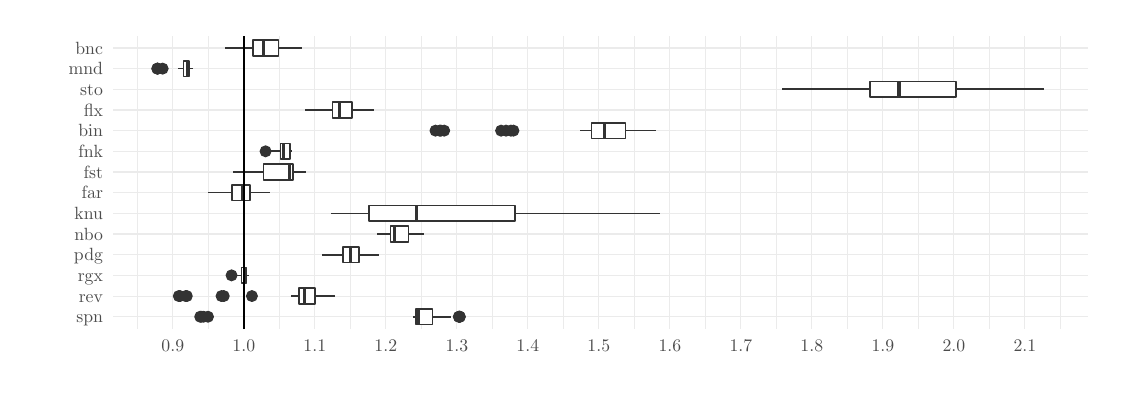
\begin{tikzpicture}[x=1pt,y=1pt]
\definecolor{fillColor}{RGB}{255,255,255}
\path[use as bounding box,fill=fillColor,fill opacity=0.00] (0,0) rectangle (390.26,130.09);
\begin{scope}
\path[clip] ( 30.80, 21.16) rectangle (383.14,127.24);
\definecolor{drawColor}{gray}{0.92}

\path[draw=drawColor,line width= 0.2pt,line join=round] ( 39.61, 21.16) --
	( 39.61,127.24);

\path[draw=drawColor,line width= 0.2pt,line join=round] ( 65.27, 21.16) --
	( 65.27,127.24);

\path[draw=drawColor,line width= 0.2pt,line join=round] ( 90.93, 21.16) --
	( 90.93,127.24);

\path[draw=drawColor,line width= 0.2pt,line join=round] (116.58, 21.16) --
	(116.58,127.24);

\path[draw=drawColor,line width= 0.2pt,line join=round] (142.24, 21.16) --
	(142.24,127.24);

\path[draw=drawColor,line width= 0.2pt,line join=round] (167.90, 21.16) --
	(167.90,127.24);

\path[draw=drawColor,line width= 0.2pt,line join=round] (193.55, 21.16) --
	(193.55,127.24);

\path[draw=drawColor,line width= 0.2pt,line join=round] (219.21, 21.16) --
	(219.21,127.24);

\path[draw=drawColor,line width= 0.2pt,line join=round] (244.87, 21.16) --
	(244.87,127.24);

\path[draw=drawColor,line width= 0.2pt,line join=round] (270.52, 21.16) --
	(270.52,127.24);

\path[draw=drawColor,line width= 0.2pt,line join=round] (296.18, 21.16) --
	(296.18,127.24);

\path[draw=drawColor,line width= 0.2pt,line join=round] (321.84, 21.16) --
	(321.84,127.24);

\path[draw=drawColor,line width= 0.2pt,line join=round] (347.50, 21.16) --
	(347.50,127.24);

\path[draw=drawColor,line width= 0.2pt,line join=round] (373.15, 21.16) --
	(373.15,127.24);

\path[draw=drawColor,line width= 0.4pt,line join=round] ( 30.80, 25.64) --
	(383.14, 25.64);

\path[draw=drawColor,line width= 0.4pt,line join=round] ( 30.80, 33.11) --
	(383.14, 33.11);

\path[draw=drawColor,line width= 0.4pt,line join=round] ( 30.80, 40.59) --
	(383.14, 40.59);

\path[draw=drawColor,line width= 0.4pt,line join=round] ( 30.80, 48.06) --
	(383.14, 48.06);

\path[draw=drawColor,line width= 0.4pt,line join=round] ( 30.80, 55.53) --
	(383.14, 55.53);

\path[draw=drawColor,line width= 0.4pt,line join=round] ( 30.80, 63.00) --
	(383.14, 63.00);

\path[draw=drawColor,line width= 0.4pt,line join=round] ( 30.80, 70.47) --
	(383.14, 70.47);

\path[draw=drawColor,line width= 0.4pt,line join=round] ( 30.80, 77.94) --
	(383.14, 77.94);

\path[draw=drawColor,line width= 0.4pt,line join=round] ( 30.80, 85.41) --
	(383.14, 85.41);

\path[draw=drawColor,line width= 0.4pt,line join=round] ( 30.80, 92.88) --
	(383.14, 92.88);

\path[draw=drawColor,line width= 0.4pt,line join=round] ( 30.80,100.35) --
	(383.14,100.35);

\path[draw=drawColor,line width= 0.4pt,line join=round] ( 30.80,107.82) --
	(383.14,107.82);

\path[draw=drawColor,line width= 0.4pt,line join=round] ( 30.80,115.29) --
	(383.14,115.29);

\path[draw=drawColor,line width= 0.4pt,line join=round] ( 30.80,122.76) --
	(383.14,122.76);

\path[draw=drawColor,line width= 0.4pt,line join=round] ( 52.44, 21.16) --
	( 52.44,127.24);

\path[draw=drawColor,line width= 0.4pt,line join=round] ( 78.10, 21.16) --
	( 78.10,127.24);

\path[draw=drawColor,line width= 0.4pt,line join=round] (103.75, 21.16) --
	(103.75,127.24);

\path[draw=drawColor,line width= 0.4pt,line join=round] (129.41, 21.16) --
	(129.41,127.24);

\path[draw=drawColor,line width= 0.4pt,line join=round] (155.07, 21.16) --
	(155.07,127.24);

\path[draw=drawColor,line width= 0.4pt,line join=round] (180.72, 21.16) --
	(180.72,127.24);

\path[draw=drawColor,line width= 0.4pt,line join=round] (206.38, 21.16) --
	(206.38,127.24);

\path[draw=drawColor,line width= 0.4pt,line join=round] (232.04, 21.16) --
	(232.04,127.24);

\path[draw=drawColor,line width= 0.4pt,line join=round] (257.70, 21.16) --
	(257.70,127.24);

\path[draw=drawColor,line width= 0.4pt,line join=round] (283.35, 21.16) --
	(283.35,127.24);

\path[draw=drawColor,line width= 0.4pt,line join=round] (309.01, 21.16) --
	(309.01,127.24);

\path[draw=drawColor,line width= 0.4pt,line join=round] (334.67, 21.16) --
	(334.67,127.24);

\path[draw=drawColor,line width= 0.4pt,line join=round] (360.32, 21.16) --
	(360.32,127.24);
\definecolor{drawColor}{gray}{0.20}
\definecolor{fillColor}{gray}{0.20}

\path[draw=drawColor,line width= 0.4pt,line join=round,line cap=round,fill=fillColor] (156.15, 25.64) circle (  1.96);

\path[draw=drawColor,line width= 0.4pt,line join=round,line cap=round,fill=fillColor] (156.12, 25.64) circle (  1.96);

\path[draw=drawColor,line width= 0.4pt,line join=round,line cap=round,fill=fillColor] (155.99, 25.64) circle (  1.96);

\path[draw=drawColor,line width= 0.4pt,line join=round,line cap=round,fill=fillColor] (155.93, 25.64) circle (  1.96);

\path[draw=drawColor,line width= 0.4pt,line join=round,line cap=round,fill=fillColor] (155.78, 25.64) circle (  1.96);

\path[draw=drawColor,line width= 0.4pt,line join=round,line cap=round,fill=fillColor] ( 65.16, 25.64) circle (  1.96);

\path[draw=drawColor,line width= 0.4pt,line join=round,line cap=round,fill=fillColor] ( 63.52, 25.64) circle (  1.96);

\path[draw=drawColor,line width= 0.4pt,line join=round,line cap=round,fill=fillColor] ( 62.73, 25.64) circle (  1.96);

\path[draw=drawColor,line width= 0.4pt,line join=round,line cap=round,fill=fillColor] ( 62.34, 25.64) circle (  1.96);

\path[draw=drawColor,line width= 0.6pt,line join=round] (146.25, 25.64) -- (152.79, 25.64);

\path[draw=drawColor,line width= 0.6pt,line join=round] (140.37, 25.64) -- (139.26, 25.64);
\definecolor{fillColor}{RGB}{255,255,255}

\path[draw=drawColor,line width= 0.6pt,line join=round,line cap=round,fill=fillColor] (146.25, 22.84) --
	(140.37, 22.84) --
	(140.37, 28.45) --
	(146.25, 28.45) --
	(146.25, 22.84) --
	cycle;

\path[draw=drawColor,line width= 1.1pt,line join=round] (141.25, 22.84) -- (141.25, 28.45);
\definecolor{fillColor}{gray}{0.20}

\path[draw=drawColor,line width= 0.4pt,line join=round,line cap=round,fill=fillColor] ( 81.03, 33.11) circle (  1.96);

\path[draw=drawColor,line width= 0.4pt,line join=round,line cap=round,fill=fillColor] ( 70.85, 33.11) circle (  1.96);

\path[draw=drawColor,line width= 0.4pt,line join=round,line cap=round,fill=fillColor] ( 70.05, 33.11) circle (  1.96);

\path[draw=drawColor,line width= 0.4pt,line join=round,line cap=round,fill=fillColor] ( 57.50, 33.11) circle (  1.96);

\path[draw=drawColor,line width= 0.4pt,line join=round,line cap=round,fill=fillColor] ( 57.11, 33.11) circle (  1.96);

\path[draw=drawColor,line width= 0.4pt,line join=round,line cap=round,fill=fillColor] ( 55.03, 33.11) circle (  1.96);

\path[draw=drawColor,line width= 0.4pt,line join=round,line cap=round,fill=fillColor] ( 54.61, 33.11) circle (  1.96);

\path[draw=drawColor,line width= 0.6pt,line join=round] (103.83, 33.11) -- (110.91, 33.11);

\path[draw=drawColor,line width= 0.6pt,line join=round] ( 98.16, 33.11) -- ( 95.23, 33.11);
\definecolor{fillColor}{RGB}{255,255,255}

\path[draw=drawColor,line width= 0.6pt,line join=round,line cap=round,fill=fillColor] (103.83, 30.31) --
	( 98.16, 30.31) --
	( 98.16, 35.92) --
	(103.83, 35.92) --
	(103.83, 30.31) --
	cycle;

\path[draw=drawColor,line width= 1.1pt,line join=round] (100.11, 30.31) -- (100.11, 35.92);
\definecolor{fillColor}{gray}{0.20}

\path[draw=drawColor,line width= 0.4pt,line join=round,line cap=round,fill=fillColor] ( 73.67, 40.59) circle (  1.96);

\path[draw=drawColor,line width= 0.6pt,line join=round] ( 79.10, 40.59) -- ( 79.80, 40.59);

\path[draw=drawColor,line width= 0.6pt,line join=round] ( 77.25, 40.59) -- ( 74.95, 40.59);
\definecolor{fillColor}{RGB}{255,255,255}

\path[draw=drawColor,line width= 0.6pt,line join=round,line cap=round,fill=fillColor] ( 79.10, 37.78) --
	( 77.25, 37.78) --
	( 77.25, 43.39) --
	( 79.10, 43.39) --
	( 79.10, 37.78) --
	cycle;

\path[draw=drawColor,line width= 1.1pt,line join=round] ( 78.68, 37.78) -- ( 78.68, 43.39);

\path[draw=drawColor,line width= 0.6pt,line join=round] (119.62, 48.06) -- (126.98, 48.06);

\path[draw=drawColor,line width= 0.6pt,line join=round] (113.92, 48.06) -- (106.44, 48.06);

\path[draw=drawColor,line width= 0.6pt,line join=round,line cap=round,fill=fillColor] (119.62, 45.25) --
	(113.92, 45.25) --
	(113.92, 50.86) --
	(119.62, 50.86) --
	(119.62, 45.25) --
	cycle;

\path[draw=drawColor,line width= 1.1pt,line join=round] (116.71, 45.25) -- (116.71, 50.86);

\path[draw=drawColor,line width= 0.6pt,line join=round] (137.64, 55.53) -- (143.32, 55.53);

\path[draw=drawColor,line width= 0.6pt,line join=round] (131.11, 55.53) -- (126.10, 55.53);

\path[draw=drawColor,line width= 0.6pt,line join=round,line cap=round,fill=fillColor] (137.64, 52.72) --
	(131.11, 52.72) --
	(131.11, 58.33) --
	(137.64, 58.33) --
	(137.64, 52.72) --
	cycle;

\path[draw=drawColor,line width= 1.1pt,line join=round] (132.52, 52.72) -- (132.52, 58.33);

\path[draw=drawColor,line width= 0.6pt,line join=round] (176.13, 63.00) -- (228.50, 63.00);

\path[draw=drawColor,line width= 0.6pt,line join=round] (123.24, 63.00) -- (109.43, 63.00);

\path[draw=drawColor,line width= 0.6pt,line join=round,line cap=round,fill=fillColor] (176.13, 60.19) --
	(123.24, 60.19) --
	(123.24, 65.80) --
	(176.13, 65.80) --
	(176.13, 60.19) --
	cycle;

\path[draw=drawColor,line width= 1.1pt,line join=round] (140.40, 60.19) -- (140.40, 65.80);

\path[draw=drawColor,line width= 0.6pt,line join=round] ( 80.43, 70.47) -- ( 87.42, 70.47);

\path[draw=drawColor,line width= 0.6pt,line join=round] ( 73.78, 70.47) -- ( 65.12, 70.47);

\path[draw=drawColor,line width= 0.6pt,line join=round,line cap=round,fill=fillColor] ( 80.43, 67.66) --
	( 73.78, 67.66) --
	( 73.78, 73.27) --
	( 80.43, 73.27) --
	( 80.43, 67.66) --
	cycle;

\path[draw=drawColor,line width= 1.1pt,line join=round] ( 77.51, 67.66) -- ( 77.51, 73.27);

\path[draw=drawColor,line width= 0.6pt,line join=round] ( 95.85, 77.94) -- (100.61, 77.94);

\path[draw=drawColor,line width= 0.6pt,line join=round] ( 85.22, 77.94) -- ( 74.17, 77.94);

\path[draw=drawColor,line width= 0.6pt,line join=round,line cap=round,fill=fillColor] ( 95.85, 75.14) --
	( 85.22, 75.14) --
	( 85.22, 80.74) --
	( 95.85, 80.74) --
	( 95.85, 75.14) --
	cycle;

\path[draw=drawColor,line width= 1.1pt,line join=round] ( 94.47, 75.14) -- ( 94.47, 80.74);
\definecolor{fillColor}{gray}{0.20}

\path[draw=drawColor,line width= 0.4pt,line join=round,line cap=round,fill=fillColor] ( 85.96, 85.41) circle (  1.96);

\path[draw=drawColor,line width= 0.6pt,line join=round] ( 94.71, 85.41) -- ( 95.48, 85.41);

\path[draw=drawColor,line width= 0.6pt,line join=round] ( 91.33, 85.41) -- ( 87.02, 85.41);
\definecolor{fillColor}{RGB}{255,255,255}

\path[draw=drawColor,line width= 0.6pt,line join=round,line cap=round,fill=fillColor] ( 94.71, 82.61) --
	( 91.33, 82.61) --
	( 91.33, 88.21) --
	( 94.71, 88.21) --
	( 94.71, 82.61) --
	cycle;

\path[draw=drawColor,line width= 1.1pt,line join=round] ( 92.53, 82.61) -- ( 92.53, 88.21);
\definecolor{fillColor}{gray}{0.20}

\path[draw=drawColor,line width= 0.4pt,line join=round,line cap=round,fill=fillColor] (175.53, 92.88) circle (  1.96);

\path[draw=drawColor,line width= 0.4pt,line join=round,line cap=round,fill=fillColor] (174.60, 92.88) circle (  1.96);

\path[draw=drawColor,line width= 0.4pt,line join=round,line cap=round,fill=fillColor] (172.86, 92.88) circle (  1.96);

\path[draw=drawColor,line width= 0.4pt,line join=round,line cap=round,fill=fillColor] (171.07, 92.88) circle (  1.96);

\path[draw=drawColor,line width= 0.4pt,line join=round,line cap=round,fill=fillColor] (150.51, 92.88) circle (  1.96);

\path[draw=drawColor,line width= 0.4pt,line join=round,line cap=round,fill=fillColor] (149.30, 92.88) circle (  1.96);

\path[draw=drawColor,line width= 0.4pt,line join=round,line cap=round,fill=fillColor] (148.89, 92.88) circle (  1.96);

\path[draw=drawColor,line width= 0.4pt,line join=round,line cap=round,fill=fillColor] (147.36, 92.88) circle (  1.96);

\path[draw=drawColor,line width= 0.6pt,line join=round] (215.97, 92.88) -- (227.06, 92.88);

\path[draw=drawColor,line width= 0.6pt,line join=round] (203.77, 92.88) -- (199.42, 92.88);
\definecolor{fillColor}{RGB}{255,255,255}

\path[draw=drawColor,line width= 0.6pt,line join=round,line cap=round,fill=fillColor] (215.97, 90.08) --
	(203.77, 90.08) --
	(203.77, 95.68) --
	(215.97, 95.68) --
	(215.97, 90.08) --
	cycle;

\path[draw=drawColor,line width= 1.1pt,line join=round] (208.57, 90.08) -- (208.57, 95.68);

\path[draw=drawColor,line width= 0.6pt,line join=round] (117.23,100.35) -- (125.27,100.35);

\path[draw=drawColor,line width= 0.6pt,line join=round] (110.12,100.35) -- (100.09,100.35);

\path[draw=drawColor,line width= 0.6pt,line join=round,line cap=round,fill=fillColor] (117.23, 97.55) --
	(110.12, 97.55) --
	(110.12,103.15) --
	(117.23,103.15) --
	(117.23, 97.55) --
	cycle;

\path[draw=drawColor,line width= 1.1pt,line join=round] (112.68, 97.55) -- (112.68,103.15);

\path[draw=drawColor,line width= 0.6pt,line join=round] (335.48,107.82) -- (367.13,107.82);

\path[draw=drawColor,line width= 0.6pt,line join=round] (304.34,107.82) -- (272.46,107.82);

\path[draw=drawColor,line width= 0.6pt,line join=round,line cap=round,fill=fillColor] (335.48,105.02) --
	(304.34,105.02) --
	(304.34,110.62) --
	(335.48,110.62) --
	(335.48,105.02) --
	cycle;

\path[draw=drawColor,line width= 1.1pt,line join=round] (314.85,105.02) -- (314.85,110.62);
\definecolor{fillColor}{gray}{0.20}

\path[draw=drawColor,line width= 0.4pt,line join=round,line cap=round,fill=fillColor] ( 48.77,115.29) circle (  1.96);

\path[draw=drawColor,line width= 0.4pt,line join=round,line cap=round,fill=fillColor] ( 47.00,115.29) circle (  1.96);

\path[draw=drawColor,line width= 0.4pt,line join=round,line cap=round,fill=fillColor] ( 46.92,115.29) circle (  1.96);

\path[draw=drawColor,line width= 0.4pt,line join=round,line cap=round,fill=fillColor] ( 46.81,115.29) circle (  1.96);

\path[draw=drawColor,line width= 0.6pt,line join=round] ( 58.27,115.29) -- ( 59.68,115.29);

\path[draw=drawColor,line width= 0.6pt,line join=round] ( 56.36,115.29) -- ( 54.49,115.29);
\definecolor{fillColor}{RGB}{255,255,255}

\path[draw=drawColor,line width= 0.6pt,line join=round,line cap=round,fill=fillColor] ( 58.27,112.49) --
	( 56.36,112.49) --
	( 56.36,118.09) --
	( 58.27,118.09) --
	( 58.27,112.49) --
	cycle;

\path[draw=drawColor,line width= 1.1pt,line join=round] ( 57.71,112.49) -- ( 57.71,118.09);

\path[draw=drawColor,line width= 0.6pt,line join=round] ( 90.59,122.76) -- ( 99.03,122.76);

\path[draw=drawColor,line width= 0.6pt,line join=round] ( 81.46,122.76) -- ( 71.38,122.76);

\path[draw=drawColor,line width= 0.6pt,line join=round,line cap=round,fill=fillColor] ( 90.59,119.96) --
	( 81.46,119.96) --
	( 81.46,125.56) --
	( 90.59,125.56) --
	( 90.59,119.96) --
	cycle;

\path[draw=drawColor,line width= 1.1pt,line join=round] ( 85.21,119.96) -- ( 85.21,125.56);
\definecolor{drawColor}{RGB}{0,0,0}

\path[draw=drawColor,line width= 0.6pt,line join=round] ( 78.10, 21.16) -- ( 78.10,127.24);
\end{scope}
\begin{scope}
\path[clip] (  0.00,  0.00) rectangle (390.26,130.09);
\definecolor{drawColor}{gray}{0.30}

\node[text=drawColor,anchor=base east,inner sep=0pt, outer sep=0pt, scale=  0.64] at ( 27.20, 23.44) {spn};

\node[text=drawColor,anchor=base east,inner sep=0pt, outer sep=0pt, scale=  0.64] at ( 27.20, 30.91) {rev};

\node[text=drawColor,anchor=base east,inner sep=0pt, outer sep=0pt, scale=  0.64] at ( 27.20, 38.38) {rgx};

\node[text=drawColor,anchor=base east,inner sep=0pt, outer sep=0pt, scale=  0.64] at ( 27.20, 45.85) {pdg};

\node[text=drawColor,anchor=base east,inner sep=0pt, outer sep=0pt, scale=  0.64] at ( 27.20, 53.32) {nbo};

\node[text=drawColor,anchor=base east,inner sep=0pt, outer sep=0pt, scale=  0.64] at ( 27.20, 60.79) {knu};

\node[text=drawColor,anchor=base east,inner sep=0pt, outer sep=0pt, scale=  0.64] at ( 27.20, 68.26) {far};

\node[text=drawColor,anchor=base east,inner sep=0pt, outer sep=0pt, scale=  0.64] at ( 27.20, 75.73) {fst};

\node[text=drawColor,anchor=base east,inner sep=0pt, outer sep=0pt, scale=  0.64] at ( 27.20, 83.20) {fnk};

\node[text=drawColor,anchor=base east,inner sep=0pt, outer sep=0pt, scale=  0.64] at ( 27.20, 90.67) {bin};

\node[text=drawColor,anchor=base east,inner sep=0pt, outer sep=0pt, scale=  0.64] at ( 27.20, 98.14) {flx};

\node[text=drawColor,anchor=base east,inner sep=0pt, outer sep=0pt, scale=  0.64] at ( 27.20,105.61) {sto};

\node[text=drawColor,anchor=base east,inner sep=0pt, outer sep=0pt, scale=  0.64] at ( 27.20,113.08) {mnd};

\node[text=drawColor,anchor=base east,inner sep=0pt, outer sep=0pt, scale=  0.64] at ( 27.20,120.55) {bnc};
\end{scope}
\begin{scope}
\path[clip] (  0.00,  0.00) rectangle (390.26,130.09);
\definecolor{drawColor}{gray}{0.30}

\node[text=drawColor,anchor=base,inner sep=0pt, outer sep=0pt, scale=  0.64] at ( 52.44, 13.15) {0.9};

\node[text=drawColor,anchor=base,inner sep=0pt, outer sep=0pt, scale=  0.64] at ( 78.10, 13.15) {1.0};

\node[text=drawColor,anchor=base,inner sep=0pt, outer sep=0pt, scale=  0.64] at (103.75, 13.15) {1.1};

\node[text=drawColor,anchor=base,inner sep=0pt, outer sep=0pt, scale=  0.64] at (129.41, 13.15) {1.2};

\node[text=drawColor,anchor=base,inner sep=0pt, outer sep=0pt, scale=  0.64] at (155.07, 13.15) {1.3};

\node[text=drawColor,anchor=base,inner sep=0pt, outer sep=0pt, scale=  0.64] at (180.72, 13.15) {1.4};

\node[text=drawColor,anchor=base,inner sep=0pt, outer sep=0pt, scale=  0.64] at (206.38, 13.15) {1.5};

\node[text=drawColor,anchor=base,inner sep=0pt, outer sep=0pt, scale=  0.64] at (232.04, 13.15) {1.6};

\node[text=drawColor,anchor=base,inner sep=0pt, outer sep=0pt, scale=  0.64] at (257.70, 13.15) {1.7};

\node[text=drawColor,anchor=base,inner sep=0pt, outer sep=0pt, scale=  0.64] at (283.35, 13.15) {1.8};

\node[text=drawColor,anchor=base,inner sep=0pt, outer sep=0pt, scale=  0.64] at (309.01, 13.15) {1.9};

\node[text=drawColor,anchor=base,inner sep=0pt, outer sep=0pt, scale=  0.64] at (334.67, 13.15) {2.0};

\node[text=drawColor,anchor=base,inner sep=0pt, outer sep=0pt, scale=  0.64] at (360.32, 13.15) {2.1};
\end{scope}
\end{tikzpicture}

  \vspace{-1cm}
  \caption{Time spent in GC}
  \label{fig:gc-time}
\end{figure}

Even an optimizing compiler has to allocate many promises for R
code, as often times, they cannot be eliminated entirely.
Thus we expect a significant portion of the speedup to originate from
the reduced allocation rate. We measured the time spent in garbage collection
and as can be seen in \autoref{fig:gc-time}, indeed a significant reduction occurs.
These numbers have to be taken with a grain of salt. The GNU R garbage
collector, which is reused in \Rsh, has a fairly slow allocation path, which
includes mutating a doubly-linked list. Therefore, some portion of the speedup
is due to the saved time in the allocation of promises, which is not counted.
Therefore, these numbers underestimate the effect on memory management overhead.
%
\begin{figure}[h]
  \centering
  % Created by tikzDevice version 0.12.3.1 on 2021-04-14 21:08:25
% !TEX encoding = UTF-8 Unicode
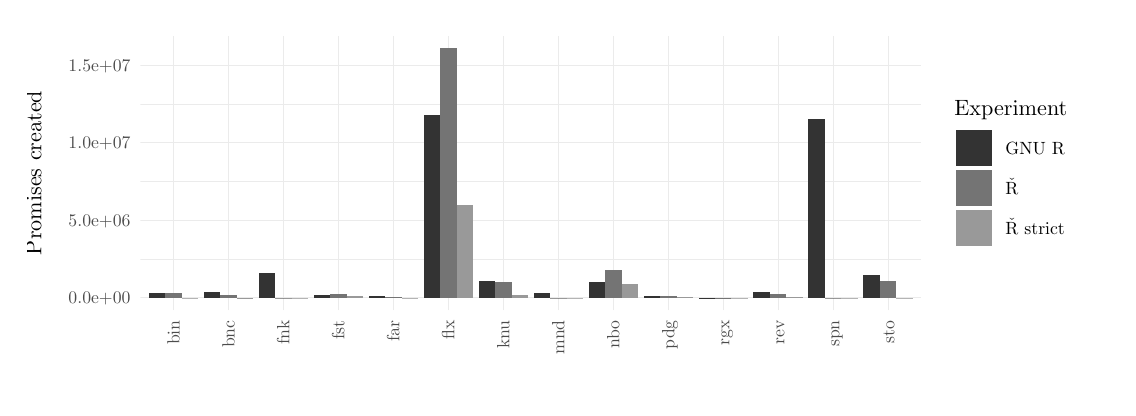
\begin{tikzpicture}[x=1pt,y=1pt]
\definecolor{fillColor}{RGB}{255,255,255}
\path[use as bounding box,fill=fillColor,fill opacity=0.00] (0,0) rectangle (390.26,130.09);
\begin{scope}
\path[clip] ( 40.75, 27.95) rectangle (322.87,127.24);
\definecolor{drawColor}{gray}{0.92}

\path[draw=drawColor,line width= 0.2pt,line join=round] ( 40.75, 46.47) --
	(322.87, 46.47);

\path[draw=drawColor,line width= 0.2pt,line join=round] ( 40.75, 74.48) --
	(322.87, 74.48);

\path[draw=drawColor,line width= 0.2pt,line join=round] ( 40.75,102.50) --
	(322.87,102.50);

\path[draw=drawColor,line width= 0.4pt,line join=round] ( 40.75, 32.46) --
	(322.87, 32.46);

\path[draw=drawColor,line width= 0.4pt,line join=round] ( 40.75, 60.48) --
	(322.87, 60.48);

\path[draw=drawColor,line width= 0.4pt,line join=round] ( 40.75, 88.49) --
	(322.87, 88.49);

\path[draw=drawColor,line width= 0.4pt,line join=round] ( 40.75,116.50) --
	(322.87,116.50);

\path[draw=drawColor,line width= 0.4pt,line join=round] ( 52.67, 27.95) --
	( 52.67,127.24);

\path[draw=drawColor,line width= 0.4pt,line join=round] ( 72.54, 27.95) --
	( 72.54,127.24);

\path[draw=drawColor,line width= 0.4pt,line join=round] ( 92.41, 27.95) --
	( 92.41,127.24);

\path[draw=drawColor,line width= 0.4pt,line join=round] (112.27, 27.95) --
	(112.27,127.24);

\path[draw=drawColor,line width= 0.4pt,line join=round] (132.14, 27.95) --
	(132.14,127.24);

\path[draw=drawColor,line width= 0.4pt,line join=round] (152.01, 27.95) --
	(152.01,127.24);

\path[draw=drawColor,line width= 0.4pt,line join=round] (171.87, 27.95) --
	(171.87,127.24);

\path[draw=drawColor,line width= 0.4pt,line join=round] (191.74, 27.95) --
	(191.74,127.24);

\path[draw=drawColor,line width= 0.4pt,line join=round] (211.61, 27.95) --
	(211.61,127.24);

\path[draw=drawColor,line width= 0.4pt,line join=round] (231.48, 27.95) --
	(231.48,127.24);

\path[draw=drawColor,line width= 0.4pt,line join=round] (251.34, 27.95) --
	(251.34,127.24);

\path[draw=drawColor,line width= 0.4pt,line join=round] (271.21, 27.95) --
	(271.21,127.24);

\path[draw=drawColor,line width= 0.4pt,line join=round] (291.08, 27.95) --
	(291.08,127.24);

\path[draw=drawColor,line width= 0.4pt,line join=round] (310.95, 27.95) --
	(310.95,127.24);
\definecolor{fillColor}{gray}{0.60}

\path[fill=fillColor] ( 75.52, 32.46) rectangle ( 81.48, 32.52);

\path[fill=fillColor] ( 75.52, 32.46) rectangle ( 81.48, 32.52);

\path[fill=fillColor] ( 75.52, 32.46) rectangle ( 81.48, 32.52);

\path[fill=fillColor] ( 75.52, 32.46) rectangle ( 81.48, 32.52);

\path[fill=fillColor] ( 75.52, 32.46) rectangle ( 81.48, 32.52);

\path[fill=fillColor] ( 75.52, 32.46) rectangle ( 81.48, 32.52);

\path[fill=fillColor] ( 75.52, 32.46) rectangle ( 81.48, 32.52);

\path[fill=fillColor] ( 75.52, 32.46) rectangle ( 81.48, 32.52);

\path[fill=fillColor] ( 75.52, 32.46) rectangle ( 81.48, 32.52);

\path[fill=fillColor] ( 75.52, 32.46) rectangle ( 81.48, 32.52);
\definecolor{fillColor}{RGB}{116,116,116}

\path[fill=fillColor] ( 69.56, 32.46) rectangle ( 75.52, 33.59);

\path[fill=fillColor] ( 69.56, 32.46) rectangle ( 75.52, 33.59);

\path[fill=fillColor] ( 69.56, 32.46) rectangle ( 75.52, 33.59);

\path[fill=fillColor] ( 69.56, 32.46) rectangle ( 75.52, 33.59);

\path[fill=fillColor] ( 69.56, 32.46) rectangle ( 75.52, 33.59);

\path[fill=fillColor] ( 69.56, 32.46) rectangle ( 75.52, 33.59);

\path[fill=fillColor] ( 69.56, 32.46) rectangle ( 75.52, 33.59);

\path[fill=fillColor] ( 69.56, 32.46) rectangle ( 75.52, 33.59);

\path[fill=fillColor] ( 69.56, 32.46) rectangle ( 75.52, 33.59);

\path[fill=fillColor] ( 69.56, 32.46) rectangle ( 75.52, 33.59);
\definecolor{fillColor}{gray}{0.20}

\path[fill=fillColor] ( 63.60, 32.46) rectangle ( 69.56, 34.54);

\path[fill=fillColor] ( 63.60, 32.46) rectangle ( 69.56, 34.54);

\path[fill=fillColor] ( 63.60, 32.46) rectangle ( 69.56, 34.54);

\path[fill=fillColor] ( 63.60, 32.46) rectangle ( 69.56, 34.54);

\path[fill=fillColor] ( 63.60, 32.46) rectangle ( 69.56, 34.54);

\path[fill=fillColor] ( 63.60, 32.46) rectangle ( 69.56, 34.54);

\path[fill=fillColor] ( 63.60, 32.46) rectangle ( 69.56, 34.54);

\path[fill=fillColor] ( 63.60, 32.46) rectangle ( 69.56, 34.54);

\path[fill=fillColor] ( 63.60, 32.46) rectangle ( 69.56, 34.54);

\path[fill=fillColor] ( 63.60, 32.46) rectangle ( 69.56, 34.54);
\definecolor{fillColor}{gray}{0.60}

\path[fill=fillColor] (194.72, 32.46) rectangle (200.68, 32.46);

\path[fill=fillColor] (194.72, 32.46) rectangle (200.68, 32.46);

\path[fill=fillColor] (194.72, 32.46) rectangle (200.68, 32.46);

\path[fill=fillColor] (194.72, 32.46) rectangle (200.68, 32.46);

\path[fill=fillColor] (194.72, 32.46) rectangle (200.68, 32.46);

\path[fill=fillColor] (194.72, 32.46) rectangle (200.68, 32.46);

\path[fill=fillColor] (194.72, 32.46) rectangle (200.68, 32.46);

\path[fill=fillColor] (194.72, 32.46) rectangle (200.68, 32.46);

\path[fill=fillColor] (194.72, 32.46) rectangle (200.68, 32.46);

\path[fill=fillColor] (194.72, 32.46) rectangle (200.68, 32.46);
\definecolor{fillColor}{RGB}{116,116,116}

\path[fill=fillColor] (188.76, 32.46) rectangle (194.72, 32.46);

\path[fill=fillColor] (188.76, 32.46) rectangle (194.72, 32.46);

\path[fill=fillColor] (188.76, 32.46) rectangle (194.72, 32.46);

\path[fill=fillColor] (188.76, 32.46) rectangle (194.72, 32.46);

\path[fill=fillColor] (188.76, 32.46) rectangle (194.72, 32.46);

\path[fill=fillColor] (188.76, 32.46) rectangle (194.72, 32.46);

\path[fill=fillColor] (188.76, 32.46) rectangle (194.72, 32.46);

\path[fill=fillColor] (188.76, 32.46) rectangle (194.72, 32.46);

\path[fill=fillColor] (188.76, 32.46) rectangle (194.72, 32.46);

\path[fill=fillColor] (188.76, 32.46) rectangle (194.72, 32.46);
\definecolor{fillColor}{gray}{0.20}

\path[fill=fillColor] (182.80, 32.46) rectangle (188.76, 34.22);

\path[fill=fillColor] (182.80, 32.46) rectangle (188.76, 34.22);

\path[fill=fillColor] (182.80, 32.46) rectangle (188.76, 34.22);

\path[fill=fillColor] (182.80, 32.46) rectangle (188.76, 34.22);

\path[fill=fillColor] (182.80, 32.46) rectangle (188.76, 34.22);

\path[fill=fillColor] (182.80, 32.46) rectangle (188.76, 34.22);

\path[fill=fillColor] (182.80, 32.46) rectangle (188.76, 34.22);

\path[fill=fillColor] (182.80, 32.46) rectangle (188.76, 34.22);

\path[fill=fillColor] (182.80, 32.46) rectangle (188.76, 34.22);

\path[fill=fillColor] (182.80, 32.46) rectangle (188.76, 34.22);
\definecolor{fillColor}{gray}{0.60}

\path[fill=fillColor] (313.93, 32.46) rectangle (319.89, 32.46);

\path[fill=fillColor] (313.93, 32.46) rectangle (319.89, 32.46);

\path[fill=fillColor] (313.93, 32.46) rectangle (319.89, 32.46);

\path[fill=fillColor] (313.93, 32.46) rectangle (319.89, 32.46);

\path[fill=fillColor] (313.93, 32.46) rectangle (319.89, 32.46);

\path[fill=fillColor] (313.93, 32.46) rectangle (319.89, 32.46);

\path[fill=fillColor] (313.93, 32.46) rectangle (319.89, 32.46);

\path[fill=fillColor] (313.93, 32.46) rectangle (319.89, 32.46);

\path[fill=fillColor] (313.93, 32.46) rectangle (319.89, 32.46);

\path[fill=fillColor] (313.93, 32.46) rectangle (319.89, 32.46);
\definecolor{fillColor}{RGB}{116,116,116}

\path[fill=fillColor] (307.97, 32.46) rectangle (313.93, 38.58);

\path[fill=fillColor] (307.97, 32.46) rectangle (313.93, 38.58);

\path[fill=fillColor] (307.97, 32.46) rectangle (313.93, 38.58);

\path[fill=fillColor] (307.97, 32.46) rectangle (313.93, 38.58);

\path[fill=fillColor] (307.97, 32.46) rectangle (313.93, 38.58);

\path[fill=fillColor] (307.97, 32.46) rectangle (313.93, 38.58);

\path[fill=fillColor] (307.97, 32.46) rectangle (313.93, 38.58);

\path[fill=fillColor] (307.97, 32.46) rectangle (313.93, 38.58);

\path[fill=fillColor] (307.97, 32.46) rectangle (313.93, 38.58);

\path[fill=fillColor] (307.97, 32.46) rectangle (313.93, 38.58);
\definecolor{fillColor}{gray}{0.20}

\path[fill=fillColor] (302.01, 32.46) rectangle (307.97, 40.88);

\path[fill=fillColor] (302.01, 32.46) rectangle (307.97, 40.88);

\path[fill=fillColor] (302.01, 32.46) rectangle (307.97, 40.88);

\path[fill=fillColor] (302.01, 32.46) rectangle (307.97, 40.88);

\path[fill=fillColor] (302.01, 32.46) rectangle (307.97, 40.88);

\path[fill=fillColor] (302.01, 32.46) rectangle (307.97, 40.88);

\path[fill=fillColor] (302.01, 32.46) rectangle (307.97, 40.88);

\path[fill=fillColor] (302.01, 32.46) rectangle (307.97, 40.88);

\path[fill=fillColor] (302.01, 32.46) rectangle (307.97, 40.88);

\path[fill=fillColor] (302.01, 32.46) rectangle (307.97, 40.88);
\definecolor{fillColor}{gray}{0.60}

\path[fill=fillColor] (154.99, 32.46) rectangle (160.95, 65.86);

\path[fill=fillColor] (154.99, 32.46) rectangle (160.95, 65.86);

\path[fill=fillColor] (154.99, 32.46) rectangle (160.95, 65.86);

\path[fill=fillColor] (154.99, 32.46) rectangle (160.95, 65.86);

\path[fill=fillColor] (154.99, 32.46) rectangle (160.95, 65.86);

\path[fill=fillColor] (154.99, 32.46) rectangle (160.95, 65.86);

\path[fill=fillColor] (154.99, 32.46) rectangle (160.95, 65.86);

\path[fill=fillColor] (154.99, 32.46) rectangle (160.95, 65.86);

\path[fill=fillColor] (154.99, 32.46) rectangle (160.95, 65.86);

\path[fill=fillColor] (154.99, 32.46) rectangle (160.95, 65.86);
\definecolor{fillColor}{gray}{0.20}

\path[fill=fillColor] (143.07, 32.46) rectangle (149.03, 98.62);

\path[fill=fillColor] (143.07, 32.46) rectangle (149.03, 98.62);

\path[fill=fillColor] (143.07, 32.46) rectangle (149.03, 98.62);

\path[fill=fillColor] (143.07, 32.46) rectangle (149.03, 98.62);

\path[fill=fillColor] (143.07, 32.46) rectangle (149.03, 98.62);

\path[fill=fillColor] (143.07, 32.46) rectangle (149.03, 98.62);

\path[fill=fillColor] (143.07, 32.46) rectangle (149.03, 98.62);

\path[fill=fillColor] (143.07, 32.46) rectangle (149.03, 98.62);

\path[fill=fillColor] (143.07, 32.46) rectangle (149.03, 98.62);

\path[fill=fillColor] (143.07, 32.46) rectangle (149.03, 98.62);
\definecolor{fillColor}{RGB}{116,116,116}

\path[fill=fillColor] (149.03, 32.46) rectangle (154.99,122.73);

\path[fill=fillColor] (149.03, 32.46) rectangle (154.99,122.73);

\path[fill=fillColor] (149.03, 32.46) rectangle (154.99,122.73);

\path[fill=fillColor] (149.03, 32.46) rectangle (154.99,122.73);

\path[fill=fillColor] (149.03, 32.46) rectangle (154.99,122.73);

\path[fill=fillColor] (149.03, 32.46) rectangle (154.99,122.73);

\path[fill=fillColor] (149.03, 32.46) rectangle (154.99,122.73);

\path[fill=fillColor] (149.03, 32.46) rectangle (154.99,122.73);

\path[fill=fillColor] (149.03, 32.46) rectangle (154.99,122.73);

\path[fill=fillColor] (149.03, 32.46) rectangle (154.99,122.73);
\definecolor{fillColor}{gray}{0.60}

\path[fill=fillColor] ( 55.65, 32.46) rectangle ( 61.61, 32.46);

\path[fill=fillColor] ( 55.65, 32.46) rectangle ( 61.61, 32.46);

\path[fill=fillColor] ( 55.65, 32.46) rectangle ( 61.61, 32.46);

\path[fill=fillColor] ( 55.65, 32.46) rectangle ( 61.61, 32.46);

\path[fill=fillColor] ( 55.65, 32.46) rectangle ( 61.61, 32.46);

\path[fill=fillColor] ( 55.65, 32.46) rectangle ( 61.61, 32.46);

\path[fill=fillColor] ( 55.65, 32.46) rectangle ( 61.61, 32.46);

\path[fill=fillColor] ( 55.65, 32.46) rectangle ( 61.61, 32.46);

\path[fill=fillColor] ( 55.65, 32.46) rectangle ( 61.61, 32.46);

\path[fill=fillColor] ( 55.65, 32.46) rectangle ( 61.61, 32.46);
\definecolor{fillColor}{RGB}{116,116,116}

\path[fill=fillColor] ( 49.69, 32.46) rectangle ( 55.65, 34.15);

\path[fill=fillColor] ( 49.69, 32.46) rectangle ( 55.65, 34.15);

\path[fill=fillColor] ( 49.69, 32.46) rectangle ( 55.65, 34.15);

\path[fill=fillColor] ( 49.69, 32.46) rectangle ( 55.65, 34.15);

\path[fill=fillColor] ( 49.69, 32.46) rectangle ( 55.65, 34.15);

\path[fill=fillColor] ( 49.69, 32.46) rectangle ( 55.65, 34.15);

\path[fill=fillColor] ( 49.69, 32.46) rectangle ( 55.65, 34.15);

\path[fill=fillColor] ( 49.69, 32.46) rectangle ( 55.65, 34.15);

\path[fill=fillColor] ( 49.69, 32.46) rectangle ( 55.65, 34.15);

\path[fill=fillColor] ( 49.69, 32.46) rectangle ( 55.65, 34.15);
\definecolor{fillColor}{gray}{0.20}

\path[fill=fillColor] ( 43.73, 32.46) rectangle ( 49.69, 34.15);

\path[fill=fillColor] ( 43.73, 32.46) rectangle ( 49.69, 34.15);

\path[fill=fillColor] ( 43.73, 32.46) rectangle ( 49.69, 34.15);

\path[fill=fillColor] ( 43.73, 32.46) rectangle ( 49.69, 34.15);

\path[fill=fillColor] ( 43.73, 32.46) rectangle ( 49.69, 34.15);

\path[fill=fillColor] ( 43.73, 32.46) rectangle ( 49.69, 34.15);

\path[fill=fillColor] ( 43.73, 32.46) rectangle ( 49.69, 34.15);

\path[fill=fillColor] ( 43.73, 32.46) rectangle ( 49.69, 34.15);

\path[fill=fillColor] ( 43.73, 32.46) rectangle ( 49.69, 34.15);

\path[fill=fillColor] ( 43.73, 32.46) rectangle ( 49.69, 34.15);
\definecolor{fillColor}{gray}{0.60}

\path[fill=fillColor] ( 95.39, 32.46) rectangle (101.35, 32.46);

\path[fill=fillColor] ( 95.39, 32.46) rectangle (101.35, 32.46);

\path[fill=fillColor] ( 95.39, 32.46) rectangle (101.35, 32.46);

\path[fill=fillColor] ( 95.39, 32.46) rectangle (101.35, 32.46);

\path[fill=fillColor] ( 95.39, 32.46) rectangle (101.35, 32.46);

\path[fill=fillColor] ( 95.39, 32.46) rectangle (101.35, 32.46);

\path[fill=fillColor] ( 95.39, 32.46) rectangle (101.35, 32.46);

\path[fill=fillColor] ( 95.39, 32.46) rectangle (101.35, 32.46);

\path[fill=fillColor] ( 95.39, 32.46) rectangle (101.35, 32.46);

\path[fill=fillColor] ( 95.39, 32.46) rectangle (101.35, 32.46);
\definecolor{fillColor}{RGB}{116,116,116}

\path[fill=fillColor] ( 89.42, 32.46) rectangle ( 95.39, 32.46);

\path[fill=fillColor] ( 89.42, 32.46) rectangle ( 95.39, 32.46);

\path[fill=fillColor] ( 89.42, 32.46) rectangle ( 95.39, 32.46);

\path[fill=fillColor] ( 89.42, 32.46) rectangle ( 95.39, 32.46);

\path[fill=fillColor] ( 89.42, 32.46) rectangle ( 95.39, 32.46);

\path[fill=fillColor] ( 89.42, 32.46) rectangle ( 95.39, 32.46);

\path[fill=fillColor] ( 89.42, 32.46) rectangle ( 95.39, 32.46);

\path[fill=fillColor] ( 89.42, 32.46) rectangle ( 95.39, 32.46);

\path[fill=fillColor] ( 89.42, 32.46) rectangle ( 95.39, 32.46);

\path[fill=fillColor] ( 89.42, 32.46) rectangle ( 95.39, 32.46);
\definecolor{fillColor}{gray}{0.20}

\path[fill=fillColor] ( 83.46, 32.46) rectangle ( 89.42, 41.37);

\path[fill=fillColor] ( 83.46, 32.46) rectangle ( 89.42, 41.37);

\path[fill=fillColor] ( 83.46, 32.46) rectangle ( 89.42, 41.37);

\path[fill=fillColor] ( 83.46, 32.46) rectangle ( 89.42, 41.37);

\path[fill=fillColor] ( 83.46, 32.46) rectangle ( 89.42, 41.37);

\path[fill=fillColor] ( 83.46, 32.46) rectangle ( 89.42, 41.37);

\path[fill=fillColor] ( 83.46, 32.46) rectangle ( 89.42, 41.37);

\path[fill=fillColor] ( 83.46, 32.46) rectangle ( 89.42, 41.37);

\path[fill=fillColor] ( 83.46, 32.46) rectangle ( 89.42, 41.37);

\path[fill=fillColor] ( 83.46, 32.46) rectangle ( 89.42, 41.37);
\definecolor{fillColor}{gray}{0.60}

\path[fill=fillColor] (115.25, 32.46) rectangle (121.21, 33.00);

\path[fill=fillColor] (115.25, 32.46) rectangle (121.21, 33.00);

\path[fill=fillColor] (115.25, 32.46) rectangle (121.21, 33.00);

\path[fill=fillColor] (115.25, 32.46) rectangle (121.21, 33.00);

\path[fill=fillColor] (115.25, 32.46) rectangle (121.21, 33.00);

\path[fill=fillColor] (115.25, 32.46) rectangle (121.21, 33.00);

\path[fill=fillColor] (115.25, 32.46) rectangle (121.21, 33.00);

\path[fill=fillColor] (115.25, 32.46) rectangle (121.21, 33.00);

\path[fill=fillColor] (115.25, 32.46) rectangle (121.21, 33.00);

\path[fill=fillColor] (115.25, 32.46) rectangle (121.21, 33.00);
\definecolor{fillColor}{gray}{0.20}

\path[fill=fillColor] (103.33, 32.46) rectangle (109.29, 33.42);

\path[fill=fillColor] (103.33, 32.46) rectangle (109.29, 33.42);

\path[fill=fillColor] (103.33, 32.46) rectangle (109.29, 33.42);

\path[fill=fillColor] (103.33, 32.46) rectangle (109.29, 33.42);

\path[fill=fillColor] (103.33, 32.46) rectangle (109.29, 33.42);

\path[fill=fillColor] (103.33, 32.46) rectangle (109.29, 33.42);

\path[fill=fillColor] (103.33, 32.46) rectangle (109.29, 33.42);

\path[fill=fillColor] (103.33, 32.46) rectangle (109.29, 33.42);

\path[fill=fillColor] (103.33, 32.46) rectangle (109.29, 33.42);

\path[fill=fillColor] (103.33, 32.46) rectangle (109.29, 33.42);
\definecolor{fillColor}{RGB}{116,116,116}

\path[fill=fillColor] (109.29, 32.46) rectangle (115.25, 33.91);

\path[fill=fillColor] (109.29, 32.46) rectangle (115.25, 33.91);

\path[fill=fillColor] (109.29, 32.46) rectangle (115.25, 33.91);

\path[fill=fillColor] (109.29, 32.46) rectangle (115.25, 33.91);

\path[fill=fillColor] (109.29, 32.46) rectangle (115.25, 33.91);

\path[fill=fillColor] (109.29, 32.46) rectangle (115.25, 33.91);

\path[fill=fillColor] (109.29, 32.46) rectangle (115.25, 33.91);

\path[fill=fillColor] (109.29, 32.46) rectangle (115.25, 33.91);

\path[fill=fillColor] (109.29, 32.46) rectangle (115.25, 33.91);

\path[fill=fillColor] (109.29, 32.46) rectangle (115.25, 33.91);
\definecolor{fillColor}{gray}{0.60}

\path[fill=fillColor] (135.12, 32.46) rectangle (141.08, 32.46);

\path[fill=fillColor] (135.12, 32.46) rectangle (141.08, 32.46);

\path[fill=fillColor] (135.12, 32.46) rectangle (141.08, 32.46);

\path[fill=fillColor] (135.12, 32.46) rectangle (141.08, 32.46);

\path[fill=fillColor] (135.12, 32.46) rectangle (141.08, 32.46);

\path[fill=fillColor] (135.12, 32.46) rectangle (141.08, 32.46);

\path[fill=fillColor] (135.12, 32.46) rectangle (141.08, 32.46);

\path[fill=fillColor] (135.12, 32.46) rectangle (141.08, 32.46);

\path[fill=fillColor] (135.12, 32.46) rectangle (141.08, 32.46);

\path[fill=fillColor] (135.12, 32.46) rectangle (141.08, 32.46);
\definecolor{fillColor}{RGB}{116,116,116}

\path[fill=fillColor] (129.16, 32.46) rectangle (135.12, 32.72);

\path[fill=fillColor] (129.16, 32.46) rectangle (135.12, 32.72);

\path[fill=fillColor] (129.16, 32.46) rectangle (135.12, 32.72);

\path[fill=fillColor] (129.16, 32.46) rectangle (135.12, 32.72);

\path[fill=fillColor] (129.16, 32.46) rectangle (135.12, 32.72);

\path[fill=fillColor] (129.16, 32.46) rectangle (135.12, 32.72);

\path[fill=fillColor] (129.16, 32.46) rectangle (135.12, 32.72);

\path[fill=fillColor] (129.16, 32.46) rectangle (135.12, 32.72);

\path[fill=fillColor] (129.16, 32.46) rectangle (135.12, 32.72);

\path[fill=fillColor] (129.16, 32.46) rectangle (135.12, 32.72);
\definecolor{fillColor}{gray}{0.20}

\path[fill=fillColor] (123.20, 32.46) rectangle (129.16, 33.15);

\path[fill=fillColor] (123.20, 32.46) rectangle (129.16, 33.15);

\path[fill=fillColor] (123.20, 32.46) rectangle (129.16, 33.15);

\path[fill=fillColor] (123.20, 32.46) rectangle (129.16, 33.15);

\path[fill=fillColor] (123.20, 32.46) rectangle (129.16, 33.15);

\path[fill=fillColor] (123.20, 32.46) rectangle (129.16, 33.15);

\path[fill=fillColor] (123.20, 32.46) rectangle (129.16, 33.15);

\path[fill=fillColor] (123.20, 32.46) rectangle (129.16, 33.15);

\path[fill=fillColor] (123.20, 32.46) rectangle (129.16, 33.15);

\path[fill=fillColor] (123.20, 32.46) rectangle (129.16, 33.15);
\definecolor{fillColor}{gray}{0.60}

\path[fill=fillColor] (174.85, 32.46) rectangle (180.81, 33.66);

\path[fill=fillColor] (174.85, 32.46) rectangle (180.81, 33.66);

\path[fill=fillColor] (174.85, 32.46) rectangle (180.81, 33.66);

\path[fill=fillColor] (174.85, 32.46) rectangle (180.81, 33.66);

\path[fill=fillColor] (174.85, 32.46) rectangle (180.81, 33.66);

\path[fill=fillColor] (174.85, 32.46) rectangle (180.81, 33.66);

\path[fill=fillColor] (174.85, 32.46) rectangle (180.81, 33.66);

\path[fill=fillColor] (174.85, 32.46) rectangle (180.81, 33.66);

\path[fill=fillColor] (174.85, 32.46) rectangle (180.81, 33.66);

\path[fill=fillColor] (174.85, 32.46) rectangle (180.81, 33.66);
\definecolor{fillColor}{RGB}{116,116,116}

\path[fill=fillColor] (168.89, 32.46) rectangle (174.85, 38.12);

\path[fill=fillColor] (168.89, 32.46) rectangle (174.85, 38.12);

\path[fill=fillColor] (168.89, 32.46) rectangle (174.85, 38.12);

\path[fill=fillColor] (168.89, 32.46) rectangle (174.85, 38.12);

\path[fill=fillColor] (168.89, 32.46) rectangle (174.85, 38.12);

\path[fill=fillColor] (168.89, 32.46) rectangle (174.85, 38.12);

\path[fill=fillColor] (168.89, 32.46) rectangle (174.85, 38.12);

\path[fill=fillColor] (168.89, 32.46) rectangle (174.85, 38.12);

\path[fill=fillColor] (168.89, 32.46) rectangle (174.85, 38.12);

\path[fill=fillColor] (168.89, 32.46) rectangle (174.85, 38.12);
\definecolor{fillColor}{gray}{0.20}

\path[fill=fillColor] (162.93, 32.46) rectangle (168.89, 38.51);

\path[fill=fillColor] (162.93, 32.46) rectangle (168.89, 38.51);

\path[fill=fillColor] (162.93, 32.46) rectangle (168.89, 38.51);

\path[fill=fillColor] (162.93, 32.46) rectangle (168.89, 38.51);

\path[fill=fillColor] (162.93, 32.46) rectangle (168.89, 38.51);

\path[fill=fillColor] (162.93, 32.46) rectangle (168.89, 38.51);

\path[fill=fillColor] (162.93, 32.46) rectangle (168.89, 38.51);

\path[fill=fillColor] (162.93, 32.46) rectangle (168.89, 38.51);

\path[fill=fillColor] (162.93, 32.46) rectangle (168.89, 38.51);

\path[fill=fillColor] (162.93, 32.46) rectangle (168.89, 38.51);
\definecolor{fillColor}{gray}{0.60}

\path[fill=fillColor] (214.59, 32.46) rectangle (220.55, 37.37);

\path[fill=fillColor] (214.59, 32.46) rectangle (220.55, 37.37);

\path[fill=fillColor] (214.59, 32.46) rectangle (220.55, 37.37);

\path[fill=fillColor] (214.59, 32.46) rectangle (220.55, 37.37);

\path[fill=fillColor] (214.59, 32.46) rectangle (220.55, 37.37);

\path[fill=fillColor] (214.59, 32.46) rectangle (220.55, 37.37);

\path[fill=fillColor] (214.59, 32.46) rectangle (220.55, 37.37);

\path[fill=fillColor] (214.59, 32.46) rectangle (220.55, 37.37);

\path[fill=fillColor] (214.59, 32.46) rectangle (220.55, 37.37);

\path[fill=fillColor] (214.59, 32.46) rectangle (220.55, 37.37);
\definecolor{fillColor}{gray}{0.20}

\path[fill=fillColor] (202.67, 32.46) rectangle (208.63, 38.35);

\path[fill=fillColor] (202.67, 32.46) rectangle (208.63, 38.35);

\path[fill=fillColor] (202.67, 32.46) rectangle (208.63, 38.35);

\path[fill=fillColor] (202.67, 32.46) rectangle (208.63, 38.35);

\path[fill=fillColor] (202.67, 32.46) rectangle (208.63, 38.35);

\path[fill=fillColor] (202.67, 32.46) rectangle (208.63, 38.35);

\path[fill=fillColor] (202.67, 32.46) rectangle (208.63, 38.35);

\path[fill=fillColor] (202.67, 32.46) rectangle (208.63, 38.35);

\path[fill=fillColor] (202.67, 32.46) rectangle (208.63, 38.35);

\path[fill=fillColor] (202.67, 32.46) rectangle (208.63, 38.35);
\definecolor{fillColor}{RGB}{116,116,116}

\path[fill=fillColor] (208.63, 32.46) rectangle (214.59, 42.41);

\path[fill=fillColor] (208.63, 32.46) rectangle (214.59, 42.41);

\path[fill=fillColor] (208.63, 32.46) rectangle (214.59, 42.41);

\path[fill=fillColor] (208.63, 32.46) rectangle (214.59, 42.41);

\path[fill=fillColor] (208.63, 32.46) rectangle (214.59, 42.41);

\path[fill=fillColor] (208.63, 32.46) rectangle (214.59, 42.41);

\path[fill=fillColor] (208.63, 32.46) rectangle (214.59, 42.41);

\path[fill=fillColor] (208.63, 32.46) rectangle (214.59, 42.41);

\path[fill=fillColor] (208.63, 32.46) rectangle (214.59, 42.41);

\path[fill=fillColor] (208.63, 32.46) rectangle (214.59, 42.41);
\definecolor{fillColor}{gray}{0.60}

\path[fill=fillColor] (234.46, 32.46) rectangle (240.42, 32.88);

\path[fill=fillColor] (234.46, 32.46) rectangle (240.42, 32.88);

\path[fill=fillColor] (234.46, 32.46) rectangle (240.42, 32.88);

\path[fill=fillColor] (234.46, 32.46) rectangle (240.42, 32.88);

\path[fill=fillColor] (234.46, 32.46) rectangle (240.42, 32.88);

\path[fill=fillColor] (234.46, 32.46) rectangle (240.42, 32.88);

\path[fill=fillColor] (234.46, 32.46) rectangle (240.42, 32.88);

\path[fill=fillColor] (234.46, 32.46) rectangle (240.42, 32.88);

\path[fill=fillColor] (234.46, 32.46) rectangle (240.42, 32.88);

\path[fill=fillColor] (234.46, 32.46) rectangle (240.42, 32.88);
\definecolor{fillColor}{RGB}{116,116,116}

\path[fill=fillColor] (228.50, 32.46) rectangle (234.46, 33.15);

\path[fill=fillColor] (228.50, 32.46) rectangle (234.46, 33.15);

\path[fill=fillColor] (228.50, 32.46) rectangle (234.46, 33.15);

\path[fill=fillColor] (228.50, 32.46) rectangle (234.46, 33.15);

\path[fill=fillColor] (228.50, 32.46) rectangle (234.46, 33.15);

\path[fill=fillColor] (228.50, 32.46) rectangle (234.46, 33.15);

\path[fill=fillColor] (228.50, 32.46) rectangle (234.46, 33.15);

\path[fill=fillColor] (228.50, 32.46) rectangle (234.46, 33.15);

\path[fill=fillColor] (228.50, 32.46) rectangle (234.46, 33.15);

\path[fill=fillColor] (228.50, 32.46) rectangle (234.46, 33.15);
\definecolor{fillColor}{gray}{0.20}

\path[fill=fillColor] (222.54, 32.46) rectangle (228.50, 33.16);

\path[fill=fillColor] (222.54, 32.46) rectangle (228.50, 33.16);

\path[fill=fillColor] (222.54, 32.46) rectangle (228.50, 33.16);

\path[fill=fillColor] (222.54, 32.46) rectangle (228.50, 33.16);

\path[fill=fillColor] (222.54, 32.46) rectangle (228.50, 33.16);

\path[fill=fillColor] (222.54, 32.46) rectangle (228.50, 33.16);

\path[fill=fillColor] (222.54, 32.46) rectangle (228.50, 33.16);

\path[fill=fillColor] (222.54, 32.46) rectangle (228.50, 33.16);

\path[fill=fillColor] (222.54, 32.46) rectangle (228.50, 33.16);

\path[fill=fillColor] (222.54, 32.46) rectangle (228.50, 33.16);
\definecolor{fillColor}{gray}{0.60}

\path[fill=fillColor] (254.32, 32.46) rectangle (260.28, 32.46);

\path[fill=fillColor] (254.32, 32.46) rectangle (260.28, 32.46);

\path[fill=fillColor] (254.32, 32.46) rectangle (260.28, 32.46);

\path[fill=fillColor] (254.32, 32.46) rectangle (260.28, 32.46);

\path[fill=fillColor] (254.32, 32.46) rectangle (260.28, 32.46);

\path[fill=fillColor] (254.32, 32.46) rectangle (260.28, 32.46);

\path[fill=fillColor] (254.32, 32.46) rectangle (260.28, 32.46);

\path[fill=fillColor] (254.32, 32.46) rectangle (260.28, 32.46);

\path[fill=fillColor] (254.32, 32.46) rectangle (260.28, 32.46);

\path[fill=fillColor] (254.32, 32.46) rectangle (260.28, 32.46);
\definecolor{fillColor}{RGB}{116,116,116}

\path[fill=fillColor] (248.36, 32.46) rectangle (254.32, 32.47);

\path[fill=fillColor] (248.36, 32.46) rectangle (254.32, 32.47);

\path[fill=fillColor] (248.36, 32.46) rectangle (254.32, 32.47);

\path[fill=fillColor] (248.36, 32.46) rectangle (254.32, 32.47);

\path[fill=fillColor] (248.36, 32.46) rectangle (254.32, 32.47);

\path[fill=fillColor] (248.36, 32.46) rectangle (254.32, 32.47);

\path[fill=fillColor] (248.36, 32.46) rectangle (254.32, 32.47);

\path[fill=fillColor] (248.36, 32.46) rectangle (254.32, 32.47);

\path[fill=fillColor] (248.36, 32.46) rectangle (254.32, 32.47);

\path[fill=fillColor] (248.36, 32.46) rectangle (254.32, 32.47);
\definecolor{fillColor}{gray}{0.20}

\path[fill=fillColor] (242.40, 32.46) rectangle (248.36, 32.47);

\path[fill=fillColor] (242.40, 32.46) rectangle (248.36, 32.47);

\path[fill=fillColor] (242.40, 32.46) rectangle (248.36, 32.47);

\path[fill=fillColor] (242.40, 32.46) rectangle (248.36, 32.47);

\path[fill=fillColor] (242.40, 32.46) rectangle (248.36, 32.47);

\path[fill=fillColor] (242.40, 32.46) rectangle (248.36, 32.47);

\path[fill=fillColor] (242.40, 32.46) rectangle (248.36, 32.47);

\path[fill=fillColor] (242.40, 32.46) rectangle (248.36, 32.47);

\path[fill=fillColor] (242.40, 32.46) rectangle (248.36, 32.47);

\path[fill=fillColor] (242.40, 32.46) rectangle (248.36, 32.47);
\definecolor{fillColor}{gray}{0.60}

\path[fill=fillColor] (274.19, 32.46) rectangle (280.15, 32.89);

\path[fill=fillColor] (274.19, 32.46) rectangle (280.15, 32.89);

\path[fill=fillColor] (274.19, 32.46) rectangle (280.15, 32.89);

\path[fill=fillColor] (274.19, 32.46) rectangle (280.15, 32.89);

\path[fill=fillColor] (274.19, 32.46) rectangle (280.15, 32.89);

\path[fill=fillColor] (274.19, 32.46) rectangle (280.15, 32.89);

\path[fill=fillColor] (274.19, 32.46) rectangle (280.15, 32.89);

\path[fill=fillColor] (274.19, 32.46) rectangle (280.15, 32.89);

\path[fill=fillColor] (274.19, 32.46) rectangle (280.15, 32.89);

\path[fill=fillColor] (274.19, 32.46) rectangle (280.15, 32.89);
\definecolor{fillColor}{RGB}{116,116,116}

\path[fill=fillColor] (268.23, 32.46) rectangle (274.19, 33.73);

\path[fill=fillColor] (268.23, 32.46) rectangle (274.19, 33.73);

\path[fill=fillColor] (268.23, 32.46) rectangle (274.19, 33.73);

\path[fill=fillColor] (268.23, 32.46) rectangle (274.19, 33.73);

\path[fill=fillColor] (268.23, 32.46) rectangle (274.19, 33.73);

\path[fill=fillColor] (268.23, 32.46) rectangle (274.19, 33.73);

\path[fill=fillColor] (268.23, 32.46) rectangle (274.19, 33.73);

\path[fill=fillColor] (268.23, 32.46) rectangle (274.19, 33.73);

\path[fill=fillColor] (268.23, 32.46) rectangle (274.19, 33.73);

\path[fill=fillColor] (268.23, 32.46) rectangle (274.19, 33.73);
\definecolor{fillColor}{gray}{0.20}

\path[fill=fillColor] (262.27, 32.46) rectangle (268.23, 34.57);

\path[fill=fillColor] (262.27, 32.46) rectangle (268.23, 34.57);

\path[fill=fillColor] (262.27, 32.46) rectangle (268.23, 34.57);

\path[fill=fillColor] (262.27, 32.46) rectangle (268.23, 34.57);

\path[fill=fillColor] (262.27, 32.46) rectangle (268.23, 34.57);

\path[fill=fillColor] (262.27, 32.46) rectangle (268.23, 34.57);

\path[fill=fillColor] (262.27, 32.46) rectangle (268.23, 34.57);

\path[fill=fillColor] (262.27, 32.46) rectangle (268.23, 34.57);

\path[fill=fillColor] (262.27, 32.46) rectangle (268.23, 34.57);

\path[fill=fillColor] (262.27, 32.46) rectangle (268.23, 34.57);
\definecolor{fillColor}{gray}{0.60}

\path[fill=fillColor] (294.06, 32.46) rectangle (300.02, 32.46);

\path[fill=fillColor] (294.06, 32.46) rectangle (300.02, 32.46);

\path[fill=fillColor] (294.06, 32.46) rectangle (300.02, 32.46);

\path[fill=fillColor] (294.06, 32.46) rectangle (300.02, 32.46);

\path[fill=fillColor] (294.06, 32.46) rectangle (300.02, 32.46);

\path[fill=fillColor] (294.06, 32.46) rectangle (300.02, 32.46);

\path[fill=fillColor] (294.06, 32.46) rectangle (300.02, 32.46);

\path[fill=fillColor] (294.06, 32.46) rectangle (300.02, 32.46);

\path[fill=fillColor] (294.06, 32.46) rectangle (300.02, 32.46);

\path[fill=fillColor] (294.06, 32.46) rectangle (300.02, 32.46);
\definecolor{fillColor}{RGB}{116,116,116}

\path[fill=fillColor] (288.10, 32.46) rectangle (294.06, 32.46);

\path[fill=fillColor] (288.10, 32.46) rectangle (294.06, 32.46);

\path[fill=fillColor] (288.10, 32.46) rectangle (294.06, 32.46);

\path[fill=fillColor] (288.10, 32.46) rectangle (294.06, 32.46);

\path[fill=fillColor] (288.10, 32.46) rectangle (294.06, 32.46);

\path[fill=fillColor] (288.10, 32.46) rectangle (294.06, 32.46);

\path[fill=fillColor] (288.10, 32.46) rectangle (294.06, 32.46);

\path[fill=fillColor] (288.10, 32.46) rectangle (294.06, 32.46);

\path[fill=fillColor] (288.10, 32.46) rectangle (294.06, 32.46);

\path[fill=fillColor] (288.10, 32.46) rectangle (294.06, 32.46);
\definecolor{fillColor}{gray}{0.20}

\path[fill=fillColor] (282.14, 32.46) rectangle (288.10, 97.03);

\path[fill=fillColor] (282.14, 32.46) rectangle (288.10, 97.03);

\path[fill=fillColor] (282.14, 32.46) rectangle (288.10, 97.03);

\path[fill=fillColor] (282.14, 32.46) rectangle (288.10, 97.03);

\path[fill=fillColor] (282.14, 32.46) rectangle (288.10, 97.03);

\path[fill=fillColor] (282.14, 32.46) rectangle (288.10, 97.03);

\path[fill=fillColor] (282.14, 32.46) rectangle (288.10, 97.03);

\path[fill=fillColor] (282.14, 32.46) rectangle (288.10, 97.03);

\path[fill=fillColor] (282.14, 32.46) rectangle (288.10, 97.03);

\path[fill=fillColor] (282.14, 32.46) rectangle (288.10, 97.03);
\end{scope}
\begin{scope}
\path[clip] (  0.00,  0.00) rectangle (390.26,130.09);
\definecolor{drawColor}{gray}{0.30}

\node[text=drawColor,anchor=base east,inner sep=0pt, outer sep=0pt, scale=  0.64] at ( 37.15, 30.26) {0.0e+00};

\node[text=drawColor,anchor=base east,inner sep=0pt, outer sep=0pt, scale=  0.64] at ( 37.15, 58.27) {5.0e+06};

\node[text=drawColor,anchor=base east,inner sep=0pt, outer sep=0pt, scale=  0.64] at ( 37.15, 86.29) {1.0e+07};

\node[text=drawColor,anchor=base east,inner sep=0pt, outer sep=0pt, scale=  0.64] at ( 37.15,114.30) {1.5e+07};
\end{scope}
\begin{scope}
\path[clip] (  0.00,  0.00) rectangle (390.26,130.09);
\definecolor{drawColor}{gray}{0.30}

\node[text=drawColor,rotate= 90.00,anchor=base east,inner sep=0pt, outer sep=0pt, scale=  0.64] at ( 54.87, 24.35) {bin};

\node[text=drawColor,rotate= 90.00,anchor=base east,inner sep=0pt, outer sep=0pt, scale=  0.64] at ( 74.74, 24.35) {bnc};

\node[text=drawColor,rotate= 90.00,anchor=base east,inner sep=0pt, outer sep=0pt, scale=  0.64] at ( 94.61, 24.35) {fnk};

\node[text=drawColor,rotate= 90.00,anchor=base east,inner sep=0pt, outer sep=0pt, scale=  0.64] at (114.48, 24.35) {fst};

\node[text=drawColor,rotate= 90.00,anchor=base east,inner sep=0pt, outer sep=0pt, scale=  0.64] at (134.34, 24.35) {far};

\node[text=drawColor,rotate= 90.00,anchor=base east,inner sep=0pt, outer sep=0pt, scale=  0.64] at (154.21, 24.35) {flx};

\node[text=drawColor,rotate= 90.00,anchor=base east,inner sep=0pt, outer sep=0pt, scale=  0.64] at (174.08, 24.35) {knu};

\node[text=drawColor,rotate= 90.00,anchor=base east,inner sep=0pt, outer sep=0pt, scale=  0.64] at (193.95, 24.35) {mnd};

\node[text=drawColor,rotate= 90.00,anchor=base east,inner sep=0pt, outer sep=0pt, scale=  0.64] at (213.81, 24.35) {nbo};

\node[text=drawColor,rotate= 90.00,anchor=base east,inner sep=0pt, outer sep=0pt, scale=  0.64] at (233.68, 24.35) {pdg};

\node[text=drawColor,rotate= 90.00,anchor=base east,inner sep=0pt, outer sep=0pt, scale=  0.64] at (253.55, 24.35) {rgx};

\node[text=drawColor,rotate= 90.00,anchor=base east,inner sep=0pt, outer sep=0pt, scale=  0.64] at (273.41, 24.35) {rev};

\node[text=drawColor,rotate= 90.00,anchor=base east,inner sep=0pt, outer sep=0pt, scale=  0.64] at (293.28, 24.35) {spn};

\node[text=drawColor,rotate= 90.00,anchor=base east,inner sep=0pt, outer sep=0pt, scale=  0.64] at (313.15, 24.35) {sto};
\end{scope}
\begin{scope}
\path[clip] (  0.00,  0.00) rectangle (390.26,130.09);
\definecolor{drawColor}{RGB}{0,0,0}

\node[text=drawColor,rotate= 90.00,anchor=base,inner sep=0pt, outer sep=0pt, scale=  0.80] at (  4.98, 77.60) {Promises created};
\end{scope}
\begin{scope}
\path[clip] (  0.00,  0.00) rectangle (390.26,130.09);
\definecolor{drawColor}{RGB}{0,0,0}

\node[text=drawColor,anchor=base west,inner sep=0pt, outer sep=0pt, scale=  0.80] at (334.87, 98.52) {Experiment};
\end{scope}
\begin{scope}
\path[clip] (  0.00,  0.00) rectangle (390.26,130.09);
\definecolor{fillColor}{gray}{0.20}

\path[fill=fillColor] (335.58, 80.00) rectangle (348.61, 93.03);
\end{scope}
\begin{scope}
\path[clip] (  0.00,  0.00) rectangle (390.26,130.09);
\definecolor{fillColor}{RGB}{116,116,116}

\path[fill=fillColor] (335.58, 65.55) rectangle (348.61, 78.58);
\end{scope}
\begin{scope}
\path[clip] (  0.00,  0.00) rectangle (390.26,130.09);
\definecolor{fillColor}{gray}{0.60}

\path[fill=fillColor] (335.58, 51.09) rectangle (348.61, 64.13);
\end{scope}
\begin{scope}
\path[clip] (  0.00,  0.00) rectangle (390.26,130.09);
\definecolor{drawColor}{RGB}{0,0,0}

\node[text=drawColor,anchor=base west,inner sep=0pt, outer sep=0pt, scale=  0.64] at (353.32, 84.31) {GNU R};
\end{scope}
\begin{scope}
\path[clip] (  0.00,  0.00) rectangle (390.26,130.09);
\definecolor{drawColor}{RGB}{0,0,0}

\node[text=drawColor,anchor=base west,inner sep=0pt, outer sep=0pt, scale=  0.64] at (353.32, 69.86) {Ř};
\end{scope}
\begin{scope}
\path[clip] (  0.00,  0.00) rectangle (390.26,130.09);
\definecolor{drawColor}{RGB}{0,0,0}

\node[text=drawColor,anchor=base west,inner sep=0pt, outer sep=0pt, scale=  0.64] at (353.32, 55.41) {Ř strict};
\end{scope}
\end{tikzpicture}

  \vspace{-1cm}
  \caption{Promises allocated}
  \label{fig:gc-pressure}
\end{figure}
%
For an additional estimation of how much promises occur and are avoided by a
strict R, we measure the number of promises allocated in the
benchmark suite per iteration for GNU R, Ř and Ř-strict. The results are shown in
\autoref{fig:gc-pressure}. The first jump from GNU R's bytecode interpreter to
the optimizing just-in-time compiler \Rsh, leads to an \promiseAlocationReductionGnurRsh
reduction in allocations. The second step
from lazy to eager semantics leads to \promiseAlocationReductionRshStrictToZero
benchmarks not allocating any promises at all. On the remainder we see an additional
\promiseAlocationReductionRshStrict reduction.
Overal, \promiseAlocationReductionRshStrictToZero benchmarks reduce to zero
allocations, the rest reduce on average by \promiseAlocationReductionGnurRshStrict.
The lowest reduction observed is
\promiseAlocationReductionGnurRshStrictMin.
Surprisingly the number of remaining promises is
still relatively high in some cases. As far as we were able to observe, they
originate largely from two sources. One are default argument expressions, which
are still bundled in promises. \OF{which bms and how much?} The other are special forms, \ie R builtins with a custom evaluation
strategy, that are not yet natively supported in the \Rsh bytecode.

\paragraph{Discussion}

It was surprising to see that the resulting speedup of both tiers were
extremely similar, however the underlying reasons were at times very different.
Take for instance the \lstinline{Binarytrees} benchmark, which showed in both
the bytecode interpreter and the native compiler a speedup of about $1.5\times$
in the strict mode. In native the execution time decreased from 79ms to 53ms, in
the interpreter from 143ms to 97ms per iteration. However, the reasons for the
seemingly similar speedup are very different. In both tiers we observed a
proportional reduction of the time spent in tracing the heap for garbage collection,
that accounted for only about $5\%$ of the speedup. We investigated the
remaining difference using \lstinline{perf} and found that for the bytecode interpreter the overheads of
lazy evaluation in that benchmark were in promise allocation (\ie acquiring an
appropriately sized chunk of memory from the freelist) and setting up the
execution context for promise evaluation. This includes marking it as being
executed to detect recursive evaluation dependencies and calling the interpreters
main eval-loop on the code of the promise.
In the native code there is also some reduction in promise allocation and
evaluation overhead, however a significant part of the speedup is due to better
optimizations. Previously the local variables of the innermost function in
that benchmark are kept in a first-class R environment, since \Rsh does not yet
support speculative environment elision for recursive functions. But thanks to eager
evaluation of the arguments, the argument promises do not leak the environment
and therefore \Rsh is able to speculatively elide it.

\section{Robustness}

For validation, we selected 2000 dependent packages of the synthesis
corpus. They have 4.5M lines of R code and 4.7M lines of native (C, C++, and
Fortran) code. We run their examples, tests, and vignettes to exercise the
functions with signatures.

% TODO for end
% Table~\cite{tab:ten_sigs} shows ten representative signatures generated by the
% synthesis step of our experiments.
%
% \begin{table}
%   \vspace{-3mm}
%   \caption{Strictness Signatures} \label{table:ten_sigs}
%   \centering
%   \begin{tabular}{ll}
%     \toprule
%     \bf Function &\bf Strictness Signature\\
%     \hline
%     \bottomrule
%   \end{tabular}
% \end{table}

\subsection{Robustness (H2)} \label{Evaluation:Robustness}

\begin{table}
  \vspace{-3mm}
  \small
  \caption{Strictness Failure} \label{table:strictfail}
  \centering
  \begin{tabular}{lcr|lr|lr|lr|lr|l}
    \toprule
    \#&\textbf{Configuration}&\multicolumn{2}{c}{\textbf{test}}&\multicolumn{2}{c}{\textbf{vignette}}&\multicolumn{2}{c}{\textbf{example}}&\multicolumn{2}{c}{\textbf{testthat}}&\multicolumn{2}{c}{\textbf{total}}\\
    \midrule
    0&$+U+E+R$&5&2.09\%&25&10.46\%&163&68.2\%&46&19.25\%&239&0.56\%\\
    1&$+U+E-R$&4&1.71\%&24&10.26\%&162&69.23\%&44&18.8\%&234&0.55\%\\
    2&$+U-E+R$&28&1.46\%&101&5.25\%&1594&82.93\%&199&10.35\%&1922&4.51\%\\
    3&$+U-E-R$&41&0.62\%&99&1.49\%&1649&24.89\%&4836&73\%&6625&15.54\%\\
    4&$-U+E+R$&21&3.44\%&87&14.26\%&409&67.05\%&93&15.25\%&610&1.43\%\\
    5&$-U+E-R$&20&3.25\%&91&14.77\%&412&66.88\%&93&15.1\%&616&1.44\%\\
    6&$-U-E+R$&46&1.98\%&156&6.73\%&1861&80.25\%&256&11.04\%&2319&5.44\%\\
    7&$-U-E-R$&57&0.8\%&181&2.53\%&2084&29.11\%&4836&67.56\%&7158&16.79\%\\
    \bottomrule
  \end{tabular}
\end{table}

\section{Discussion}



\section{Migration Strategy}
- py2to3 does not do a good job
- hack has a simple migration tool
- scala 2 to 3 has migration tools

- If we have signatures for every test on CRAN.
-
\AG{rlang has defiintion of SEXP.}

%%\section*{Acknowledgments}
%% TODO: Thank Flip
\bibliography{bib/jv, bib/aviral, bib/ml, bib/bib}

\end{document}
